% 第 6 章 缝合解
% 来源：[KneserPaper] §3.3（Welding construction）、§6（W2）、§7（W1）、§8（char）、Remark paulsen；
%       sec-general.tex 的改写清单；docs/theory-core-zh.md §2；docs/quad-kneser-zh.md §4。
% 本章新宏（\providecommand，名字带特征前缀以免与他章冲突）：
\providecommand{\WienerA}{\mathfrak A}          % 加权 Wiener 代数 𝔄_H
\providecommand{\Tcirc}{T^{\circ}}               % T° = T − id − t₀
\providecommand{\Pineg}{\Pi_{<0}}                % 负模投影
\providecommand{\Pinonneg}{\Pi_{\ge 0}}          % 非负模投影
\providecommand{\Csew}{\mathcal C}               % 类 𝒞(Y)
\providecommand{\etwopi}[1]{\ee^{2\pi\ii #1}}    % e^{2πi·}
\providecommand{\Rtime}{\mathcal R}              % 吸引时间（R⁻¹ 的一个分支）
\providecommand{\Stime}{\mathcal S}              % 排斥时间（S⁻¹ 的一个分支）
\providecommand{\Band}{\mathcal B}               % 带状透镜 𝓑_s(Y)

\chapter{缝合解}\label{ch:sewing}

前两章给出了两个吸引、排斥正则解 $R,S$ 和它们之间的转移映射 $T=R^{-1}\circ S$。
任何一个「上方用 $R$ 表示、下方用 $S$ 表示」的分数迭代，其分离系数都由 $T$ 决定（\cref{thm:welding}）。
但到目前为止，我们还不知道这样的分数迭代是否存在，也不知道它是否唯一。

本章回答这两个问题。构造是几何的：把 $R$ 的上半柱面和 $S$ 的下半柱面沿 $T-\ii h$ 共形缝合，
缝出的曲面同构于 $\C^*$，它的万有覆叠坐标给出一个分数迭代 $\Ksew$，称为\textbf{缝合解}（sewing solution）。
为了得到定量信息，我们再用加权 Wiener 代数中的一个压缩映射把同一个解构造一遍。
压缩给出 $c_n/\Lam^n-\tau_n=O(\Lam)$，常数只依赖于族。
最后我们证明：在「缝口高度条件」规定的类中，缝合解是唯一的；这个条件是一个选根条件，不能去掉。

\begin{goals}
\item 两个半柱面沿 $T-\ii h$ 的共形焊接给出 $\C^*$，从而给出缝合解 $\Ksew$（\cref{ch6:prop:weld}）。
\item 加权 Wiener 代数 $\WienerA_H$ 中的压缩 $\mathcal T(Q)=-\Pineg[\Tcirc\circ(\id+Q)]$ 构造 $\Ksew$，
  并给出 $|c_n/\Lam^n-\tau_n|\le C_n\Lam$（\cref{thm:sewing}）。
\item $\Ksew$ 对开折参数全纯依赖；$\Ima s<0$ 时它在 $\pm\ii\infty$ 分别趋于两个不动点（\cref{ch6:thm:parameter}）。
\item 类 $\Csew(Y)$ 与刻画定理：$\Csew(Y)=\{\Ksew\}$（\cref{def:class,thm:characterization}）；
  缝口高度条件排除了平移解 $\Ksew(\cdot+c_j)$。
\item 一阶修正：在 (H5) 下 $\hat c_1/\tau_1-1=\Lam[-4\pi^2|\tau_1|^2-2\pi\ii\tau_1-4\pi\ii\tau_2\bar\tau_1/\tau_1]+O(\Lam^2)$，
  以及它的数值检验（\cref{ch6:prop:first-correction}）。
\end{goals}

\section{设定与回顾}\label{ch6:sec:setup}

本章始终在下面的设定中工作。

\paragraph{族与尺度.}
$f_s$ 是满足 (H1)--(H4) 的实鞍结开折（\cref{def:unfolding}），$s>0$ 一侧有两个实不动点。
$u$ 是仿射坐标 $w=w^*+cu$；为了书写简单，本章取 $c=1$，即 $u=w-w^*$
（对 tetration 取 $c=\ee$ 时只需把下文的 $w^*+u_j$ 换成 $w^*+\ee u_j$，估计不变）。在 $u$ 坐标下仍把映射写成 $f_s$。吸引、排斥不动点为 $u_1<u_2$，乘子 $0<\lambda_1<1<\lambda_2$，
留数 $A_j=1/\log\lambda_j$，周期 $h=2\pi/|\log\lambda_1|$、$h_2=2\pi/\log\lambda_2$，强迫尺度 $\Lam=\ee^{-2\pi h}$。
由 \cref{prop:scales} 与 \cref{lem:residues}，当 $s\to0^+$ 时
\begin{gather}\label{ch6:eq:scales}
 |\log\lambda_1|,\ \log\lambda_2=2\sqrt{a_2\gamma s}\,\bigl(1+O(\sqrt s)\bigr),\\
 A_1+A_2\to\rho,\qquad A_1(u_1-u_2)\to\frac1{a_2},\qquad h_2-h\to2\pi\rho .\notag
\end{gather}
特别地 $h\to\infty$，$\Lam\to0$，并且 $|u_1|,|u_2|\le C|\log\lambda_1|$。
本章所有「常数」都只依赖于族（即依赖于 $f_s(w)$ 在 $(s,w)=(0,w^*)$ 附近的芽和基点 $w_0$），不依赖于 $s$；
$C$ 表示这样的常数，每次出现可以不同。

\paragraph{两个正则解与转移映射.}
吸引正则解 $R(z)=\sigma^{-1}(\sigma(w_0)\lambda_1^{z})$（\cref{def:regular-solution}），$R(0)=w_0$，
以 $\ii h$ 为周期（因为 $\lambda_1^{\ii h}=\ee^{\ii h\log\lambda_1}=\ee^{-2\pi\ii}=1$）。它满足
\begin{equation}\label{ch6:eq:sigmaR}
 \sigma\bigl(R(w)\bigr)=\sigma(w_0)\,\lambda_1^{w},
\end{equation}
只要左边有定义。$R$ 不是整函数：$\sigma^{-1}$ 只能沿 $f_s$ 的逆分支延拓，$R$ 在一个闭集 $\Sigma_R$ 外全纯，
$\Sigma_R$ 由 $f_s$ 的奇异值经逆分支拉回得到（对 tetration，$\Sigma_R=\bigcup_k((-\infty,-2]+\ii kh)$）。
排斥正则解 $S(z)=\sigma_{\mathrm{rep}}^{-1}(-\lambda_2^{z})$ 由 (H1) 延拓为整函数，以 $\ii h_2$ 为周期，
把 $\R$ 递减地映到 $(w^*+u_1,w^*+u_2)$ 上（\cref{def:transition}）。

转移映射 $T=R^{-1}\circ S$ 取 \cref{lem:realT} 的分支：$\Ima t_0=h/2$。于是
\begin{equation}\label{ch6:eq:Treal}
 T(z)-z=\sum_{n\in\Z}t_n\etwopi{nz},\qquad T(x)-x-\tfrac{\ii h}2\in\R\ (x\in\R),\qquad t_{-n}=\overline{t_n},
\end{equation}
$\tau_n=t_n\etwopi{(-nt_0)}$，$\Tcirc=T-\id-t_0$。因为 $|\etwopi{t_0}|=\ee^{-2\pi\Ima t_0}=\ee^{-\pi h}=\Lam^{1/2}$，
\begin{equation}\label{ch6:eq:tn-size}
 |t_n|=|\tau_n|\,\Lam^{n/2}\qquad(n\ge1).
\end{equation}
所以只要 $\tau_n$ 有界（第 7 章证明它们收敛），$T$ 的非零模就是指数小的。
本章不用第 7 章的收敛结果；我们直接从带状区域上的估计得到 $t_n$ 的一致上界（\cref{ch6:lem:modes}）。

\paragraph{解与分离系数.}
\textbf{解}（solution）指一个在某闭集（\textbf{奇异集}，singular set）之外全纯、并在有定义处满足
\begin{equation}\label{ch6:eq:abel}
 K(z+1)=f_s\bigl(K(z)\bigr)
\end{equation}
的函数（这里 $f_s$ 写在 $w$ 坐标下）。若 $K=R\circ(\id+P)$ 在一个上半平面上成立，其中 $P$ 是有界、全纯、$1$-周期的，
那么在 $q=\etwopi{z}$ 下 $P$ 是穿孔圆盘上的有界全纯函数，$q=0$ 是可去奇点，所以
\begin{equation}\label{ch6:eq:P-expansion}
 P(z)=\sum_{n\ge0}c_n\etwopi{nz},\qquad P(z)\to c_0\quad(\Ima z\to+\infty).
\end{equation}
$c_n$ 是\textbf{分离系数}（separation coefficients），$\hat c_n=c_n/\Lam^n$，$\Xi_n=c_n/c_1^n$。同理，下半平面上有界周期的 $Q$ 只有非正模。
这个「有界周期函数只有单侧模」的事实本章会反复使用。

\section{共形焊接}\label{ch6:sec:weld}

\subsection{缝合曲面}

\begin{proposition}[焊接]\label{ch6:prop:weld}
设 $s>0$ 足够小。取两个半柱面
\[
 C_-=\{\Ima w'\le0\}/\Z\quad(\text{排斥时间}),\qquad
 C_+=\{\Ima w\ge-h/2\}/\Z\quad(\text{吸引时间}),
\]
把 $C_-$ 的边界与 $C_+$ 的边界按 $w=T(w')-\ii h$ 等同。
\begin{enumerate}
\item 得到的曲面 $X$ 是一个 Riemann 曲面，且 $X\cong\C^*$。
\item 设 $z$ 是 $X$ 的万有覆叠坐标，选成使覆叠变换为 $z\mapsto z+1$、且上端对应 $\Ima z\to+\infty$。那么
 \[
  K(z)=R\bigl(w(z)\bigr)\ \ (\text{$z$ 在 $C_+$ 的提升中}),\qquad K(z)=S\bigl(w'(z)\bigr)\ \ (\text{$z$ 在 $C_-$ 的提升中})
 \]
 是 \eqref{ch6:eq:abel} 的解，在 $w(z)\in\Sigma_R$ 的点之外全纯。
\item $w(z)-z$ 是 $1$-周期的，在上端附近只有非负模；$w'(z)-z$ 是 $1$-周期的，在下端附近只有非正模。
 坐标 $z$ 在相差一个平移的意义下唯一。
\end{enumerate}
\end{proposition}

\begin{proof}
(1) 由 \eqref{ch6:eq:Treal}，$T(x)-\ii h$ 的虚部恒为 $-h/2$，所以 $T-\ii h$ 把 $C_-$ 的边界圆 $\R/\Z$ 映到 $C_+$ 的边界圆
$(\R-\ii h/2)/\Z$。由 \cref{lem:realT}(3)，$T(x+1)=T(x)+1$，$T'(x)>0$，并且 $T-\ii h$ 把 $\R$ 双射地映到 $\R-\ii h/2$
（$T'>0$ 的来源是：$S'<0$，而 $(R^{-1})'=\sigma'/(\sigma\log\lambda_1)$ 在线段 $(w^*+u_1,w^*+u_2)$ 上也为负）。
所以粘合映射是边界圆之间保向的实解析微分同胚，并延拓为边界附近的全纯映射。
在边界的一个邻域内用这个全纯延拓作为坐标变换，$X$ 就有了复结构。

$X$ 在拓扑上是一个开柱面。它的两端是穿孔圆盘：上端用坐标 $\etwopi{w}$（$\Ima w\to+\infty$），下端用 $\etwopi{(-w')}$。
补上两个点后得到单连通的紧 Riemann 曲面，由单值化定理它是 $\widehat\C$。去掉两点，$X\cong\C^*$。

(2) 在缝上两个定义一致：$R(T(w')-\ii h)=R(T(w'))=S(w')$，因为 $\ii h$ 是 $R$ 的周期，并且 $R\circ T=S$。
$\pi_1(X)\cong\Z$ 的生成元提升为 $z\mapsto z+1$，在两个图上分别作用为 $w\mapsto w+1$、$w'\mapsto w'+1$，
所以 $K(z+1)=R(w+1)=f_s(R(w))=f_s(K(z))$，下方同理（$S(w'+1)=f_s(S(w'))$）。

(3) 在上端附近，$q=\etwopi{z}$ 与 $\etwopi{w}$ 都是 $X$ 的穿孔圆盘坐标，并且都在该端趋于 $0$；
它们之间的坐标变换是穿孔圆盘之间的双全纯映射，把穿孔映到穿孔，因此是在 $0$ 处有单零点的全纯函数：
$\etwopi{w}=q\,\exp(\text{$q$ 的全纯函数})$。取对数即知 $w-z$ 是 $q$ 的全纯函数，只有非负模。下端同理。
$\C^*$ 的保持两端的自同构是 $q\mapsto\alpha q$，所以 $z$ 唯一到相差平移。
\end{proof}

\begin{definition}[缝合解]\label{ch6:def:sewn}
在 \cref{ch6:prop:weld} 中，$0\in\C$ 落在 $C_+$ 内部（因为 $0>-h/2$）。
选坐标 $z$ 使 $z=0$ 对应 $C_+$ 中的点 $w=0$，并且 $w(z)=z+P(z)$，$P$ 有界周期、$P(0)=0$。
所得的解记为 $\Ksew=\Ksew_s$，称为\textbf{缝合解}。它满足 $\Ksew(0)=R(0)=w_0$。
\end{definition}

\begin{remark}\label{ch6:rem:normalisation}
「$\Ksew(0)=w_0$」本身并不确定平移：$C_+$ 中的点 $w=\ii jh$（$j\ge1$）也被 $R$ 映到 $w_0$。
\cref{ch6:def:sewn} 用的是更细的归一化：标记点是 $C_+$ 中的 $w=0$ 这一个点。
\cref{ch6:sec:char} 会说明：选错标记点得到的平移解 $\Ksew(\cdot+c_j)$ 正是缝口高度条件要排除的东西。
\end{remark}

\begin{remark}[奇异集]\label{ch6:rem:singular}
$S$ 是整函数，而 $R$ 不是，所以 $\Ksew$ 的奇异集全部来自上方的 $R$ 表示：它是 $w^{-1}(\Sigma_R)$。
对 tetration，除了 $(-\infty,-2]$ 附近的割线，还有 $(-\infty,-2]+\ii kh$（$k\ge1$）附近的副本落在 $R$ 表示的区域里。
\end{remark}

由 \cref{ch6:prop:weld}(3)，$\Ksew$ 满足 \cref{thm:welding} 的假设（上方 $\varphi_+=w$，下方 $\varphi_-=w'$），
所以它的分离系数由焊接恒等式与 $T$ 的 Fourier 系数相联系。\Cref{ch6:sec:contraction} 把这个联系定量化。

\begin{figure}[htbp]
\centering
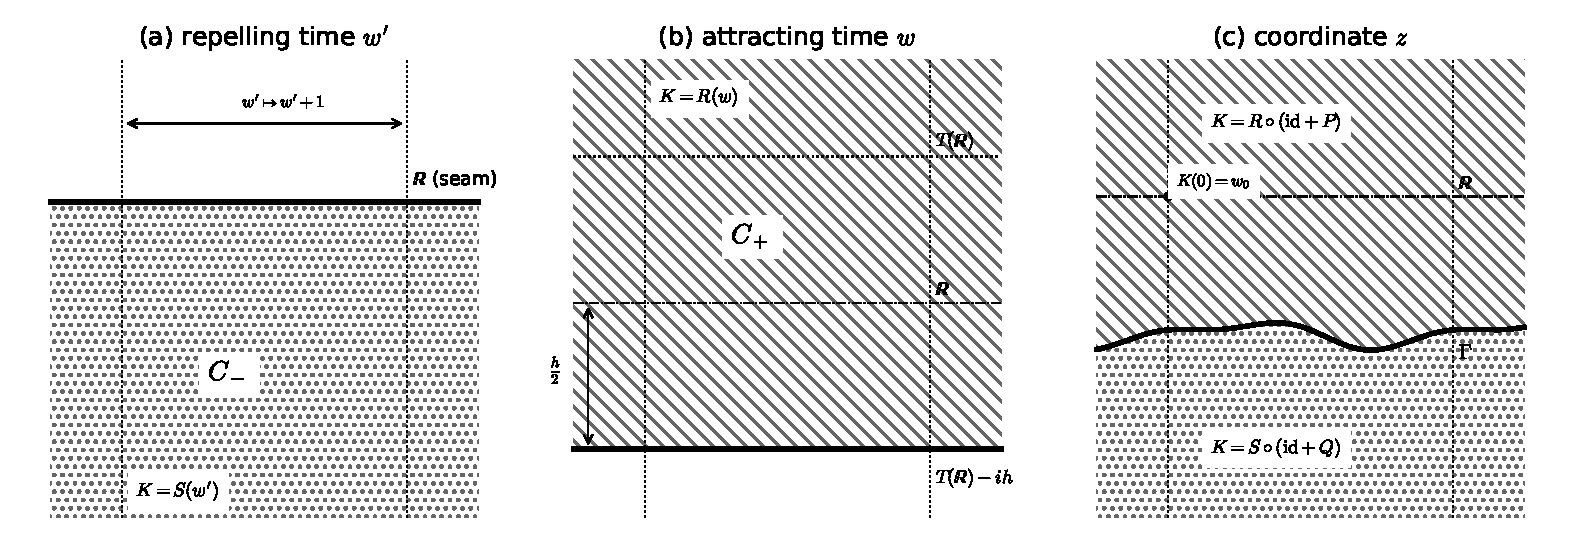
\includegraphics[width=\textwidth]{figures/fig6_welding.pdf}
\caption{缝合解的焊接示意（脚本 \texttt{figures/fig6\_welding.py}）。(a) 排斥时间 $w'$ 中的下半柱面 $C_-$，缝是实轴；
(b) 吸引时间 $w$ 中的上半柱面 $C_+$，缝是直线 $\Ima w=-h/2$，它是 $\R$ 在 $T-\ii h$ 下的像；
点线 $T(\R)$ 在实轴上方半个周期处。(c) 单值化坐标 $z$：缝 $\Gamma$ 是 $\Ima z\approx-h/2$ 附近的一条曲线，
上方 $K=R\circ(\id+P)$，下方 $K=S\circ(\id+Q)$，$K(0)=w_0$。虚线是基本域的边界。}
\label{ch6:fig:welding}
\end{figure}

\subsection{参数依赖：Fischer--Grauert 论证}

缝合解是用单值化定义的，单值化映射对参数的依赖并不自动全纯。下面的论证对每个固定的 $s_0$ 都成立，但不给出一致的估计。

\begin{proposition}[缝合族的局部参数依赖]\label{ch6:prop:weld-family}
设 $s_0>0$ 足够小。则存在复圆盘 $\Delta\ni s_0$，使 \cref{ch6:def:sewn} 的缝合解延拓为 $\Delta$ 上的全纯族：
在万有覆叠坐标的每个公共正则区域上，$\Ksew_s(z)$ 对 $(s,z)$ 联合全纯，$\Ksew_s(0)=w_0$。
不同 $s_0$ 的局部族在重叠处一致，因而定义在 $(0,s_1)$ 的一个复邻域上（这里不断言邻域的宽度一致）。
\end{proposition}

\begin{proof}
两个不动点及其 Koenigs 坐标在 $s_0$ 附近全纯依赖于 $s$。紧集 $S_{s_0}([0,1])\subset(w^*+u_1,w^*+u_2)$ 在吸引域内且不含不动点，
所以所选的 $T_s=R_s^{-1}\circ S_s$ 的分支在「参数圆盘 $\times$ $[0,1]$ 附近的窄带」上联合全纯；
$T_s(w'+1)=T_s(w')+1$ 把它延拓到整条带。\Cref{ch6:prop:weld} 的证明说明 $T_{s_0}'>0$ 在 $\R$ 上成立。
由紧性与局部单射性，存在更窄的带使 $T_{s_0}$ 在其上模 $1$ 单射；缩小参数圆盘后这一性质保持，
并且实圆周的像是柱面中的解析 Jordan 曲线。

令 $U_s=T_s+\varpi_s$，$\varpi_s=2\pi\ii/\log\lambda_1(s)$ 是 $R_s$ 的周期；在实的 $s$ 处 $\varpi_s=-\ii h$，$U_s=T_s-\ii h$。
取小的 $\delta>0$，排斥图 $\{\Ima w'<\delta/2\}/\Z$ 和吸引图「曲线 $U_s(\{\Ima w'=-\delta/2\})$ 上方」的区域，
在 $|\Ima w'|<\delta/2$ 上用 $(s,w')\mapsto(s,U_s(w'))$ 等同。缩小参数圆盘后，这些图与坐标变换构成一个 Hausdorff 的全纯柱面族；
在 $s=s_0$ 处它就是 \cref{ch6:prop:weld} 的焊接（用解析领口代替边界）。用与参数无关的局部坐标 $\etwopi{w}$、$\etwopi{(-w')}$ 补上两端，
得到一个真的全纯淹没，纤维是亏格 $0$ 的紧 Riemann 曲面。两个补上的点与上图中的点 $w=0$ 是三个互不相交的全纯截面
（缩小圆盘后 $w=0$ 留在缝的上方）。

纤维两两双全纯的真全纯族是局部全纯平凡的（Fischer--Grauert 定理~\cite{FischerGrauert1965}）。
再用逐纤维的唯一 Möbius 变换把三个截面送到 $0,\infty,1$，得到在紧化纤维上联合全纯的坐标 $q_s$。
取局部提升 $z=(2\pi\ii)^{-1}\log q_s$，使标记点 $w=0$ 对应 $z=0$。在重叠区的提升上，$R_s(U_s(w'))=S_s(w')$，
因为 $\varpi_s$ 是 $R_s$ 的周期。所以两个正则解定义了 $\Ksew_s$，它在两个表示正则处联合全纯，且 $\Ksew_s(0)=R_s(0)=w_0$。
在实参数上这正是 \cref{ch6:def:sewn} 的焊接。标记坐标使局部族唯一，由恒等定理它们在重叠圆盘上拼接。
\end{proof}

\Cref{ch6:thm:parameter} 会在 $s\to0^+$ 的一侧给出定量的版本：压缩的常数与 $s_0$ 无关，但参数圆盘的大小仍不作一致的断言。

\section{带状区域与转移映射的模}\label{ch6:sec:band}

为了把焊接写成一个压缩问题，需要知道 $T$ 在多宽的带上全纯、以及 $\Tcirc$ 在带上有多小。
本节的估计只用到第 4 章的尺度，不用第 7 章的汇流定理。

\subsection{模型时间与一步误差}

由 Weierstrass 预备定理（\cref{thm:weierstrass-prep}），存在固定的 $r>0$，使 $s$ 小时
\begin{equation}\label{ch6:eq:prepared}
 f_s(u)-u=(u-u_1)(u-u_2)\,k_s(u)\qquad(|u|<r),
\end{equation}
$k_s$ 在 $D_r$ 上全纯、无零点，并一致收敛到 $k_0(u)=(g(u)-u)/u^2=a_2+a_3u+\cdots$。定义\textbf{模型时间}（model time）与两个辅助函数
\[
 \Psi_s(u)=A_1\log(u-u_1)+A_2\log(u-u_2),\qquad
 F_s=\Psi_s\circ f_s-\Psi_s-1,\qquad
 Z_s(u)=A_1\log\frac{u-u_1}{u-u_2}.
\]
$\Psi_s$ 是一个向量场的时间函数，它的时间 $1$ 映射在 $u_1,u_2$ 处的乘子正是 $\lambda_1,\lambda_2$；$F_s$ 衡量 $f_s$ 偏离这个时间 $1$ 映射的程度。

\begin{lemma}[一步误差]\label{ch6:lem:model}
存在 $r'\in(0,r)$ 与常数 $M_1$，使 $s$ 小时：
\begin{enumerate}
\item $F_s$ 在 $D_{r'}$ 上单值全纯，且 $|F_s(u)|\le M_1|u-u_1|\,|u-u_2|$（$u\in D_{r'/2}$）；
\item $Z_s\circ f_s-Z_s$ 在 $D_{r'}$ 上单值全纯，且 $Z_s(f_s(u))-Z_s(u)=1+O(|u|+|\log\lambda_1|)$ 在 $D_{r'/2}$ 上一致成立。
\end{enumerate}
\end{lemma}

\begin{proof}
由 \eqref{ch6:eq:prepared}，$(f(u)-u_1)/(u-u_1)=1+(u-u_2)k(u)$，$(f(u)-u_2)/(u-u_2)=1+(u-u_1)k(u)$，所以
\[
 F=A_1\log\frac{1+(u-u_2)k}{1+(u-u_1)k}+(A_1+A_2)\log\bigl(1+(u-u_1)k\bigr)-1 ,
\]
$r'$ 小时对数的自变量接近 $1$，取主支，$F$ 单值全纯。第一个对数是 $O(|u_1-u_2|)$，而 $A_1(u_1-u_2)$ 与 $A_1+A_2$ 有界（\eqref{ch6:eq:scales}），
所以在 $|u|=r'$ 上 $|F|\le M_0$，$M_0$ 不依赖于 $s$。在 $u=u_1$ 处第一项是 $A_1\log\lambda_1=1$，第二项为 $0$，故 $F(u_1)=0$；
在 $u=u_2$ 处 $F(u_2)=-A_1\log\lambda_2+(A_1+A_2)\log\lambda_2-1=A_2\log\lambda_2-1=0$。
于是 $F/((u-u_1)(u-u_2))$ 在 $D_{r'}$ 上全纯，由最大模原理，它在 $D_{r'}$ 上不超过 $M_0/(r'/2)^2$（当 $|u_j|<r'/2$）。取 $M_1=4M_0/r'^2$。

(2) $Z(f(u))-Z(u)=A_1[\log(1+(u-u_2)k)-\log(1+(u-u_1)k)]=A_1(u_1-u_2)k(u)\,(1+O(|u|+|u_1|+|u_2|))$。
又 $\lambda_1=1+(u_1-u_2)k(u_1)$ 给出 $A_1(u_1-u_2)=1/k(u_1)+O(|u_1-u_2|)$，而 $k(u)/k(u_1)=1+O(|u-u_1|)$。
再用 $|u_j|\le C|\log\lambda_1|$。
\end{proof}

\begin{remark}
第 7 章的汇流定理用的是同样的两个估计（见 \cref{lem:petal}）：沿吸引轨道 $\Ima Z$ 基本不动、$\Rea Z$ 每步增加约 $1$，
而 $\sum_k|F(f^ku)|$ 一致可和。这里我们把它们用在一个不同的区域上：两个不动点之间的「透镜」。
\end{remark}

\subsection{透镜}

在 $\C\setminus((-\infty,u_1]\cup[u_2,\infty))$ 上取 $Z_s$ 的分支使 $\Ima Z_s\in(0,h)$。
在线段 $(u_1,u_2)$ 上 $(u-u_1)/(u-u_2)<0$，这一分支给出 $\Ima Z_s=h/2$；在 $\Ima u>0$ 上 $\Ima Z_s<h/2$。对 $Y>0$ 令
\[
 \Band_s(Y)=\{u:\ Y<\Ima Z_s(u)<h-Y\},
\]
它是以 $u_1,u_2$ 为角点、由两条圆弧围成的透镜，包含线段 $(u_1,u_2)$。记
\[
 c_\rho:=\pi|\rho|+1 .
\]

\begin{lemma}[透镜]\label{ch6:lem:band}
存在常数 $Y_B\ge8$，使对 $Y_B\le Y\le h/2$ 与所有足够小的 $s>0$：
\begin{enumerate}
\item 每个 $u\in\Band_s(Y)$ 的前向轨道留在 $D_{r'}$ 中并趋于 $u_1$，主后向轨道留在 $D_{r'}$ 中并趋于 $u_2$，且
 \[
  \sum_{k\in\Z}|F_s(f_s^ku)|\le\frac CY+C|\log\lambda_1| ;
 \]
\item 吸引时间与实归一化排斥时间
 \[
  \Rtime_s=\Psi_s+\sum_{k\ge0}F_s\circ f_s^k+c_R,\qquad \Stime_s=\Psi_s-\sum_{k\ge1}F_s\circ f_s^{-k}+c_S
 \]
 在 $\Band_s(Y)$ 上全纯且单射。适当选取常数 $c_R,c_S$ 后，$\Rtime_s$ 是 $R^{-1}$ 的分支（与 \cref{lem:realT} 所选分支一致），
 $\Stime_s$ 是 $S^{-1}$ 的分支，在 $(u_1,u_2)$ 上取实值，并且
 \begin{equation}\label{ch6:eq:ImS}
  \bigl|\Ima\Stime_s(u)-(\Ima Z_s(u)-h/2)\bigr|\le\pi|\rho|+\frac CY+C|\log\lambda_1|+o(1)\qquad(s\to0^+);
 \end{equation}
\item $S$ 把带 $\Sigma=\{|\Ima w'|<h/2-Y-c_\rho\}$ 映入 $\Band_s(Y)$，且 $\Stime_s\circ S=\id$。因此 $T=\Rtime_s\circ S$ 在 $\Sigma$ 上全纯，且
 \begin{equation}\label{ch6:eq:Tsum}
  T(w')-w'=(c_R-c_S)+\sum_{k\in\Z}F_s\bigl(f_s^k(S(w'))\bigr).
 \end{equation}
\end{enumerate}
\end{lemma}

\begin{proof}
(i) 令 $q=(u-u_1)/(u-u_2)=\ee^{Z/A_1}$，$\zeta=Z/A_1=-|\log\lambda_1|Z$。在透镜上 $\Ima\zeta\in(-2\pi+|\log\lambda_1|Y,\,-|\log\lambda_1|Y)$。
在 $-2\pi\le\Ima\zeta\le0$ 上，$\ee^\zeta-1$ 只有零点 $0$ 和 $-2\pi\ii$，并有初等不等式
$|\ee^\zeta-1|\ge c\min(1,\delta(\zeta))\max(1,|\ee^\zeta|)$，其中 $\delta(\zeta)=\min(|\zeta|,|\zeta+2\pi\ii|)$，$c>0$ 是绝对常数。
在透镜上 $\delta(\zeta)=|\log\lambda_1|\min(|Z|,|Z-\ii h|)>|\log\lambda_1|Y$。由 $u-u_2=(u_2-u_1)/(q-1)$ 和 $|u_2-u_1|\le C|\log\lambda_1|$ 得
\begin{gather}\label{ch6:eq:bandsize}
 |u-u_2|\le C\Bigl(|\log\lambda_1|+\frac1Y\Bigr),\\
 |u-u_1||u-u_2|=\frac{|q|\,|u_2-u_1|^2}{|q-1|^2}\le
 \begin{cases}C\min(|Z|,|Z-\ii h|)^{-2},&\delta(\zeta)\le1,\\[2pt]
 C|\log\lambda_1|^2\,\ee^{-|\log\lambda_1|\,|\Rea Z|},&\delta(\zeta)>1,\end{cases}
\end{gather}
这里用了 $|q|/\max(1,|q|)^2=\ee^{-|\Rea\zeta|}$。所以 $Y$ 大、$s$ 小时 $\Band_s(Y)\subset D_{r'/2}$。
由 \cref{ch6:lem:model}(2)，只要轨道留在 $D_{r'/2}$ 中，$\Rea Z$ 每步至少增加 $\tfrac34$。

虚部通过 $\Psi_s=Z_s+(A_1+A_2)\log(u-u_2)$ 控制：$\Psi_s(f(u))=\Psi_s(u)+1+F_s(u)$。
沿轨道 $u_k=f^ku$ 有 $\Rea Z(u_k)\ge\Rea Z(u_0)+\tfrac34k$，代入 \eqref{ch6:eq:bandsize}：
$\delta(\zeta_k)\le1$ 的点贡献至多 $C\sum_k(x_k^2+Y^2)^{-1}\le C/Y$（$x_k=\Rea Z(u_k)$ 的间距至少 $\tfrac34$，而 $\min(|Z|,|Z-\ii h|)^2\ge x^2+Y^2$），
其余的点贡献至多 $C|\log\lambda_1|^2\sum_k\ee^{-|\log\lambda_1||x_k|}\le C|\log\lambda_1|$。由 \cref{ch6:lem:model}(1)，$\sum_k|F(u_k)|\le C/Y+C|\log\lambda_1|$。
另一方面 $\Ima Z-\Ima\Psi=-(A_1+A_2)\arg(u-u_2)$，$\arg(u-u_2)\in(0,2\pi)$ 在透镜上成立。所以沿轨道 $\Ima Z$ 的漂移至多
$C/Y+C|\log\lambda_1|+2\pi|A_1+A_2|$。取 $Y_B\ge\max(8,\,8\pi|\rho|+8,\,C)$，则 $s$ 小时它小于 $1+1+2\pi|\rho|+1<Y/2$。
归纳可知轨道留在 $\Band_s(Y/2)\subset D_{r'/2}$ 中，$\Rea Z(u_k)\to+\infty$，即 $u_k\to u_1$；
沿轨道延拓的 $Z$ 值虚部在 $(Y/2,h-Y/2)\subset(0,h)$ 中，所以与固定的割平面分支一致。

后向轨道是\textbf{反射逆族}（reflected inverse family）$G_s(v)=-f_s^{-1}(-v)$ 的前向轨道。它在 $(0,0)$ 附近联合全纯，芽为 $v+a_2v^2+(2a_2^2-a_3)v^3+\cdots$，
迭代留数为 $-\rho$，吸引不动点 $-u_2$ 的乘子为 $1/\lambda_2$，其周期为 $h_2=h+2\pi\rho+o(1)$（\eqref{ch6:eq:scales}）。
$G_s$ 的 $Z$ 函数是 $(A_2/A_1)Z_s(-v)$ 加上一个分支常数，$|A_2/A_1|=h_2/h$，所以对 $Y\le h/2$，
$\Band_s(Y)$ 包含在 $G_s$ 的高度至少为 $Y-\pi|\rho|-1$ 的透镜中。增大 $Y_B$ 后同样的论证适用。

(ii) 前向轨道上 $\Psi_s(f^nu)-n=A_1\log\sigma(f^nu)+A_2\log(f^nu-u_2)-n+o(1)=A_1\log\sigma(u)+A_2\log(u_1-u_2)+o(1)$，
因为 $\sigma(f^nu)=\lambda_1^n\sigma(u)$、$A_1\log\lambda_1=1$、$\sigma'(u_1)=1$。所以 $\Rtime_s=\lim_n[\Psi_s(f^nu)-n]+c_R$
等于 $A_1\log\sigma$ 加常数，即 $R^{-1}$ 的一个分支加常数；取 $c_R$ 使它与 \cref{lem:realT} 的分支一致
（$\Band_s(Y)$ 单连通，$\sigma$ 在其上无零点：若 $f^n(u)=u_1$，由 $f$ 在 $D_{r'}$ 上单射得 $u=u_1$，而 $u_1\notin\Band_s(Y)$）。
同理 $\Stime_s$ 是 $A_2\log(-\sigma_{\mathrm{rep}})$ 加常数。$F_s$ 与 $f_s$ 是实的，所以两个级数在线段上取实值。
在线段上 $\Ima Z=h/2$、$\arg(u-u_2)=\pi$，选 $\Ima c_S$ 使 $\Stime_s$ 在线段上为实，再选 $\Rea c_S$ 使 $\Stime_s\circ S(0)=0$。于是
\[
 \Ima\Stime_s-(\Ima Z-h/2)=(A_1+A_2)\bigl(\arg(u-u_2)-\pi\bigr)-\Ima\sum_{k\ge1}F_s(f_s^{-k}u),
\]
由 $|A_1+A_2|\le|\rho|+o(1)$ 与 (i) 得 \eqref{ch6:eq:ImS}。
单射性：若 $\Stime_s(u)=\Stime_s(u')$，则主后向轨道满足 $\sigma_{\mathrm{rep}}(u_{-n})=\sigma_{\mathrm{rep}}(u'_{-n})$，$n$ 大时它们在 $u_2$ 附近，
$\sigma_{\mathrm{rep}}$ 在那里单射，故 $u_{-n}=u'_{-n}$。$f_s$ 在 $D_{r'}$ 上单射（由 $f_0'(w^*)=1$，缩小 $r'$ 即可），所以 $u=u'$。
$\Rtime_s$ 的单射性同理，用 $\sigma$ 和前向轨道。

(iii) 固定 $x\in\R$。$S(x)\in(u_1,u_2)\subset\Band_s(Y)$，且 $\Stime_s(S(x))=x$（两者都是 $A_2\log(-\sigma_{\mathrm{rep}}\circ S)$ 加常数，常数已由归一化确定）。
让 $y'$ 从 $0$ 移向 $\pm(h/2-Y-c_\rho)$。只要 $S(x+\ii y')$ 留在透镜中，解析延拓给出 $\Stime_s(S(x+\ii y'))=x+\ii y'$。
它不能从角点 $u_1,u_2$ 离开，因为在角点附近 $|\Rea\Stime_s|\to\infty$，而 $x$ 固定。它也不能从圆弧离开：
在圆弧上 $\Ima Z\in\{Y,h-Y\}$，由 \eqref{ch6:eq:ImS}，$|\Ima\Stime_s|\ge h/2-Y-\pi|\rho|-C/Y-C|\log\lambda_1|-o(1)>h/2-Y-c_\rho>|y'|$。
所以 $S(\Sigma)\subset\Band_s(Y)$，$\Stime_s\circ S=\id$。在实轴上 $T=R^{-1}\circ S=\Rtime_s\circ S$，由解析延拓这在 $\Sigma$ 上成立。
最后 $T(w')-w'=\Rtime_s(u)-\Stime_s(u)$（$u=S(w')$），这就是 \eqref{ch6:eq:Tsum}。
\end{proof}

\begin{remark}\label{ch6:rem:band-const}
论文 \cite{KneserPaper} 对 tetration 取 $\rho=\tfrac13$，那里 \eqref{ch6:eq:ImS} 的常数是 $\pi/3$，带 $\Sigma$ 的半宽取 $h/2-Y-2$。
一般情形 $\pi|\rho|$ 可以大于 $2$，所以这里用 $c_\rho=\pi|\rho|+1$ 代替 $2$。这只改变常数 $Y_0$ 的值。
\end{remark}

\subsection{模的一致估计}

\begin{lemma}[模的一致上界]\label{ch6:lem:modes}
令 $Y_0:=Y_B+1+c_\rho$，$d:=h/2-Y_0-1$。存在 $s_1>0$ 与常数 $M\le1$，使对 $0<s<s_1$：
$T$ 在带 $\{|\Ima w'|<d+1\}$ 上全纯，在闭带 $\{|\Ima w'|\le d+\tfrac12\}$ 上 $|\Tcirc|\le M$，从而
\[
 |t_n|\le M\,\ee^{-2\pi|n|(d+1/2)}\le M\,\ee^{-2\pi|n|d}\qquad(n\ne0).
\]
\end{lemma}

\begin{proof}
在 \cref{ch6:lem:band}(iii) 中取 $Y=Y_B+1$，于是 \eqref{ch6:eq:ImS} 在透镜的闭包上可用。$\Sigma$ 的半宽为 $h/2-Y_B-1-c_\rho=d+1$。
由 \eqref{ch6:eq:Tsum} 与 (i)，$T-\id=(c_R-c_S)+\Theta$，其中 $|\Theta|\le C/Y_B+C|\log\lambda_1|$。$t_0$ 是 $T-\id$ 在一条水平线上的平均，
所以 $|\Tcirc|=|\Theta-\text{平均}|\le2(C/Y_B+C|\log\lambda_1|)$ 在 $\Sigma$ 上成立。取 $M$ 为它在 $0<s<s_1$ 上的上确界；
增大 $Y_B$、缩小 $s_1$ 可使 $M\le1$。对 $n>0$ 在直线 $\Ima w'=d+\tfrac12$ 上、对 $n<0$ 在 $\Ima w'=-(d+\tfrac12)$ 上用 Cauchy 估计
$t_n=\int_0^1\Tcirc(x+\ii y)\etwopi{(-n(x+\ii y))}\,\dd x$。这里没有用到第 7 章。
\end{proof}

注意 $d=h/2-Y_0-1$，所以 $\ee^{-2\pi d}=\Lam^{1/2}\ee^{2\pi(Y_0+1)}$。\Cref{ch6:lem:modes} 说的是
\[
 |t_n|\le M\ee^{2\pi|n|(Y_0+1)}\Lam^{|n|/2},
\]
这与 \eqref{ch6:eq:tn-size} 一致，但它不需要知道 $\tau_n$ 有界。

\section{Wiener 代数中的压缩}\label{ch6:sec:contraction}

\subsection{加权 Wiener 代数}

\begin{definition}\label{ch6:def:wiener}
对 $H>0$，$\WienerA_H$（\textbf{加权 Wiener 代数}，weighted Wiener algebra）是 $1$-周期函数 $g=\sum_{n\in\Z}g_n\etwopi{nz}$ 组成的空间，范数
\[
 \|g\|_H=\sum_{n\in\Z}|g_n|\,\ee^{2\pi|n|H}<\infty .
\]
$\Pineg$、$\Pinonneg$ 分别是到负模、非负模的投影：$\Pineg g=\sum_{n<0}g_n\etwopi{nz}$，$\Pinonneg g=g-\Pineg g$。
\end{definition}

\begin{lemma}\label{ch6:lem:wiener}
\begin{enumerate}
\item $\WienerA_H$ 是 Banach 代数：$\|g_1g_2\|_H\le\|g_1\|_H\|g_2\|_H$。
\item $g\in\WienerA_H$ 在闭带 $|\Ima z|\le H$ 上连续、在开带上全纯，且 $\sup_{|\Ima z|\le H}|g|\le\|g\|_H$；
 每个系数满足 $|g_k|\le\|g\|_H\,\ee^{-2\pi|k|H}$。
\item $\Pineg$、$\Pinonneg$ 的范数为 $1$；$\Pineg\WienerA_H$ 是闭子空间。
\item $\|\ee^{g}\|_H\le\ee^{\|g\|_H}$，$\|\ee^{g}-1\|_H\le\|g\|_H\ee^{\|g\|_H}$，$\|\ee^{g_1}-\ee^{g_2}\|_H\le\|g_1-g_2\|_H\,\ee^{\max_j\|g_j\|_H}$。
\item 若 $g\in\Pineg\WienerA_H$，则 $\ee^{g}-1\in\Pineg\WienerA_H$；特别地 $[\ee^g]_0=1$，$[\ee^g]_k=0$（$k>0$），并且 $g^j$ 只有 $\le-j$ 的模。
\end{enumerate}
\end{lemma}

\begin{proof}
(1) 权是次可乘的：$\ee^{2\pi|n+m|H}\le\ee^{2\pi|n|H}\ee^{2\pi|m|H}$，所以 Cauchy 乘积的范数不超过范数之积。
(2) 在 $|\Ima z|\le H$ 上 $|\etwopi{nz}|=\ee^{-2\pi n\Ima z}\le\ee^{2\pi|n|H}$，级数绝对一致收敛。系数估计由范数定义直接得到。
(3) 显然。(4) 由 (1) 逐项估计指数级数；第三个不等式用 $\ee^{g_1}-\ee^{g_2}=(g_1-g_2)\int_0^1\ee^{tg_1+(1-t)g_2}\dd t$。
(5) 负模函数的乘积仍只有负模，模的下标相加。
\end{proof}

\subsection{缝合定理}

固定 $\beta=\tfrac14$。设 $M,d$ 如 \cref{ch6:lem:modes}，取常数 $D\ge1$ 使
\begin{equation}\label{ch6:eq:Dchoice}
 4\pi M\,\ee^{-2\pi D}\le\beta\,(1-\ee^{-2\pi D})^2 ,
\end{equation}
并令
\[
 H=d-D-\beta=\frac h2-Y_0-1-D-\beta,\qquad C_1=4M+2\beta,\qquad \varepsilon_0=C_1\Lam\,\ee^{4\pi(Y_0+D+1)} .
\]
下面的定理把焊接写成两个周期函数 $\varphi_\pm$：$\varphi_-$ 是下方的 $S$ 时间，$\varphi_+-\ii h$ 是上方的 $R$ 时间，缝的方程是 $\varphi_+=T\circ\varphi_-$。
未知的是 $\varphi_-=\id+Q$，$Q$ 只有负模（保证它在下端是坐标变换）；而 $\varphi_+-\id$ 只能有非负模。把 $T\circ(\id+Q)$ 的负模清零，就是下面的不动点方程。

\begin{theorem}[缝合定理]\label{thm:sewing}
设 \textup{(H1)--(H4)} 成立。存在 $s_1>0$，使对 $0<s<s_1$ 有 $H>1$、$\varepsilon_0<\tfrac12$，并且：
\begin{enumerate}
\item 映射 $\mathcal T(Q)=-\Pineg[\Tcirc\circ(\id+Q)]$ 把球 $\mathbb B=\{Q\in\Pineg\WienerA_H:\|Q\|_H\le\beta\}$ 映入自身，
 并且是压缩常数不超过 $\tfrac12$ 的压缩。它的不动点 $Q^*$ 与 $P':=\Pinonneg[\Tcirc\circ(\id+Q^*)]$ 满足
 \begin{equation}\label{ch6:eq:seam}
  T\circ(\id+Q^*)=\id+t_0+P'\qquad(|\Ima z|<H).
 \end{equation}
\item $\varphi_-=\id+Q^*$ 在 $\{\Ima z<H-1\}$ 上单叶，$\varphi_+=\id+t_0+P'$ 在 $\{\Ima z>-(H-1)\}$ 上单叶。
 在上方等于 $R\circ(\varphi_+-\ii h)$、下方等于 $S\circ\varphi_-$ 的函数是 \eqref{ch6:eq:abel} 的解，
 它就是 \cref{ch6:prop:weld} 的缝合解（相差平移）。
\item 方程 $\varphi_+(z_0)=\ii h$ 在圆盘 $|z-(\ii h-t_0)|<1$ 中有唯一解 $z_0$，且 $|z_0-(\ii h-t_0)|\le\varepsilon_0$。
 平移 $z\mapsto z+z_0$ 后得到 \cref{ch6:def:sewn} 的 $\Ksew$：$\Ksew(0)=w_0$，$P=R^{-1}\circ\Ksew-\id$ 满足 $P(0)=0$。
\item 对每个 $n\ge1$，$P$ 的 Fourier 系数满足
 \[
  \Bigl|\frac{c_n}{\Lam^n}-\tau_n\Bigr|\le C_n\Lam,\qquad C_n=C\,M(M+1)\,\ee^{2\pi(n+2)(Y_0+D+2)},
 \]
 其中 $C$ 是绝对常数。常数 $Y_B,Y_0,D,M$ 只依赖于族。
\end{enumerate}
\end{theorem}

\begin{proof}
$s_1$ 的选取：$d\sim\pi/|\log\lambda_1|\to\infty$，$\Lam\to0$，所以 $s$ 小时 $H>1$、$\varepsilon_0<\tfrac12$。

(1) 先说明复合有意义。$Q\in\mathbb B$ 时 $|Q|\le\beta$，于是在 $|\Ima z|\le H$ 上 $|\Ima(z+Q(z))|\le H+\beta=d-D<d$，
落在 $T$ 的全纯带内（\cref{ch6:lem:modes}），$T$ 在那里等于它的 Fourier 级数。所以
\[
 \Tcirc\circ(\id+Q)=\sum_{m\ne0}t_m\,\etwopi{mz}\,\etwopi{mQ},
\]
右边在 $\WienerA_H$ 中绝对收敛：由 \cref{ch6:lem:wiener}(4)，$\|\etwopi{mQ}\|_H\le\ee^{2\pi|m|\beta}$，故
\[
 \|\Tcirc\circ(\id+Q)\|_H\le\sum_{m\ne0}|t_m|\,\ee^{2\pi|m|(H+\beta)}\le2M\sum_{m\ge1}\ee^{-2\pi mD}=\frac{2M\ee^{-2\pi D}}{1-\ee^{-2\pi D}}
 \le\frac{\beta(1-\ee^{-2\pi D})}{2\pi}\le\beta ,
\]
这里用了 $|t_m|\le M\ee^{-2\pi|m|d}$、$d-H-\beta=D$ 与 \eqref{ch6:eq:Dchoice}。因为 $\Pineg$ 的范数为 $1$，$\mathcal T(\mathbb B)\subset\mathbb B$。同样，
\[
 \begin{aligned}
 \|\Tcirc\circ(\id+Q_1)-\Tcirc\circ(\id+Q_2)\|_H&\le\sum_{m\ne0}|t_m|\ee^{2\pi|m|(H+\beta)}\,2\pi|m|\,\|Q_1-Q_2\|_H\\
 &\le\frac{4\pi M\ee^{-2\pi D}}{(1-\ee^{-2\pi D})^2}\|Q_1-Q_2\|_H\le\beta\|Q_1-Q_2\|_H .
 \end{aligned}
\]
$\beta=\tfrac14\le\tfrac12$。$\mathbb B$ 是完备度量空间的闭子集，由压缩映射原理有唯一不动点 $Q^*$。
把 $\Tcirc\circ(\id+Q^*)$ 分成非负模和负模两部分：$\Tcirc\circ(\id+Q^*)=P'+\Pineg[\cdots]=P'-Q^*$，即 \eqref{ch6:eq:seam}。

(2) $Q^*$ 只有负模，$|q_k|\le\beta\ee^{-2\pi|k|H}$，所以它的级数在整个 $\{\Ima z\le H\}$ 上收敛（对负模，$|\etwopi{kz}|=\ee^{2\pi|k|\Ima z}$），
且在那里 $|Q^*|\le\beta$。在 $\Ima z\le H-1$ 上，
$|{Q^*}'(z)|\le\sum_{k<0}2\pi|k|\ee^{-2\pi|k|}\cdot|q_k|\ee^{2\pi|k|H}\le2\pi\max_{k\ge1}(k\ee^{-2\pi k})\,\|Q^*\|_H\le2\pi\ee^{-2\pi}\beta<1$，
所以 $\Rea\varphi_-'>0$。在凸区域上导数实部为正的全纯函数是单叶的（Noshiro--Warschawski：$\varphi(z_2)-\varphi(z_1)=(z_2-z_1)\int_0^1\varphi'(z_1+t(z_2-z_1))\dd t$，积分的实部为正）。
$\|P'\|_H\le\beta$，同样的论证给出 $\varphi_+$ 在上方的单叶性。

在重叠带 $|\Ima z|<H-1$ 上，由 \eqref{ch6:eq:seam}，
$R\circ(\varphi_+-\ii h)=R\circ(T\circ\varphi_--\ii h)=R\circ T\circ\varphi_-=S\circ\varphi_-$，
因为 $\ii h$ 是 $R$ 的周期，并且 $R\circ T=S$ 在 $\varphi_-$ 的取值处成立（这些值在 \cref{ch6:lem:band} 的带 $\Sigma$ 中，那里 $T=\Rtime_s\circ S$，$\Rtime_s$ 是 $R^{-1}$ 的分支）。
所以两个表示拼成一个函数；$\varphi_\pm$ 与 $z\mapsto z+1$ 交换，故它满足 \eqref{ch6:eq:abel}。

它实现了 \cref{ch6:prop:weld} 的焊接。令 $\Gamma=\varphi_-^{-1}(\R)$，这是 $|\Ima z|\le\beta$ 中的一条周期曲线
（$\varphi_-$ 单叶，$|\Ima\varphi_--\Ima z|\le\beta$）。因为 $\varphi_\pm-\id$ 有界，在大的基本矩形边界上用辐角原理可知：
$\varphi_-$ 把 $\Gamma$ 下方映满 $\{\Ima w'<0\}$，$\varphi_+-\ii h=T\circ\varphi_--\ii h$ 把 $\Gamma$ 映到 $T(\R)-\ii h=\{\Ima w=-h/2\}$，
并把 $\Gamma$ 上方映满 $\{\Ima w>-h/2\}$。于是 $z$ 是缝合曲面的单值化坐标，由 \cref{ch6:prop:weld}(3) 的唯一性，所得的解是缝合解的平移。

(3) 记 $P'=\sum_{n\ge0}p'_n\etwopi{nz}$，则 $|p'_n|\le\beta\ee^{-2\pi nH}$。
由 \cref{ch6:lem:wiener}(5)，$[\etwopi{mQ^*}]_k=0$（$k>0$）、$[\etwopi{mQ^*}]_0=1$，所以在 $\Tcirc\circ(\id+Q^*)$ 中只有 $m\ge1$ 的项贡献非负模：
\begin{equation}\label{ch6:eq:pn}
 p'_n=\sum_{m\ge\max(n,1)}t_m\,[\etwopi{mQ^*}]_{n-m}\qquad(n\ge0).
\end{equation}
对 $n=0$：$|[\etwopi{mQ^*}]_{-m}|\le\ee^{2\pi m\beta}\ee^{-2\pi mH}$，故
\[
 |p'_0|\le\sum_{m\ge1}M\ee^{-2\pi m(d+H-\beta)}\le2M\ee^{-2\pi(d+H-\beta)}=2M\Lam\,\ee^{2\pi(2Y_0+2+D+2\beta)}.
\]
在 $\Ima z\ge h/2-1$ 上，$|P'(z)-p'_0|\le\sum_{n\ge1}\beta\ee^{-2\pi nH}\ee^{-2\pi n(h/2-1)}\le2\beta\Lam\,\ee^{2\pi(Y_0+D+2+\beta)}$，
因为 $H+h/2-1=h-(Y_0+D+2+\beta)$。由 $D\ge1\ge2\beta$，两者之和不超过 $(2M+2\beta)\Lam\ee^{4\pi(Y_0+D+1)}\le\varepsilon_0$。

令 $z_c=\ii h-t_0$，$\Ima z_c=h/2$。在圆盘 $|z-z_c|\le1$ 上，$\varphi_+(z)-\ii h=(z-z_c)+E(z)$，$E=p'_0+(P'-p'_0)$，$|E|\le\varepsilon_0<\tfrac12$。
在圆周 $|z-z_c|=1$ 上 $|E|<|z-z_c|$，由 Rouché 定理 $\varphi_+-\ii h$ 在圆盘内恰有一个零点 $z_0$，且 $|z_0-z_c|=|E(z_0)|\le\varepsilon_0$。
于是 $R(\varphi_+(z_0)-\ii h)=R(0)=w_0$。平移后，$P(z)=\varphi_+(z+z_0)-\ii h-z$，$P(0)=0$。
$z=0$ 对应上图中 $w=\varphi_+(z_0)-\ii h=0$ 的点，所以这正是 \cref{ch6:def:sewn} 的归一化。

(4) 平移后 $P$ 的第 $n$ 个模是 $c_n=p'_n\etwopi{nz_0}$。由 \eqref{ch6:eq:pn}，$n\ge1$ 时
\[
 |p'_n-t_n|\le\sum_{m>n}M\ee^{-2\pi md}\ee^{2\pi m\beta}\ee^{-2\pi(m-n)H}\le2M\,\ee^{-2\pi n(d-\beta)}\,\ee^{-2\pi(d+H-\beta)} .
\]
写 $z_0=\ii h-t_0+\zeta$，$|\zeta|\le\varepsilon_0$。则 $\etwopi{nz_0}=\Lam^n\etwopi{(-nt_0)}\etwopi{n\zeta}$，从而
\begin{equation}\label{ch6:eq:chat-split}
 \frac{c_n}{\Lam^n}-\tau_n=\tau_n\bigl(\etwopi{n\zeta}-1\bigr)+(p'_n-t_n)\,\etwopi{(-nt_0)}\,\etwopi{n\zeta}.
\end{equation}
由 $|\etwopi{(-nt_0)}|=\ee^{\pi nh}$ 与 $d=h/2-Y_0-1$：$|\tau_n|=|t_n|\ee^{\pi nh}\le M\ee^{2\pi n(Y_0+1)}$，
$|(p'_n-t_n)\etwopi{(-nt_0)}|\le2M\ee^{2\pi n(Y_0+1+\beta)}\Lam\,\ee^{2\pi(2Y_0+2+D+2\beta)}$。

若 $2\pi n|\zeta|\le1$，则 $|\etwopi{n\zeta}-1|\le2\pi\ee n|\zeta|\le2\pi\ee nC_1\Lam\ee^{4\pi(Y_0+D+1)}$，$|\etwopi{n\zeta}|\le\ee$。
\eqref{ch6:eq:chat-split} 的第一项不超过 $2\pi\ee\,nMC_1\Lam\,\ee^{2\pi n(Y_0+1)+4\pi(Y_0+D+1)}$，第二项不超过
$2\ee M\Lam\,\ee^{2\pi[n(Y_0+1+\beta)+2Y_0+2+D+2\beta]}$。因为 $n\le\ee^{2\pi n}$、$C_1\le4(M+1)$，并且
$n(Y_0+1+\beta)+2Y_0+2+D+2\beta\le(n+2)(Y_0+D+2)$、$n(Y_0+2)+2(Y_0+D+1)\le(n+2)(Y_0+D+2)$，两项都不超过 $\tfrac12C_n\Lam$。

若 $2\pi n|\zeta|>1$，则 $1<2\pi nC_1\Lam\ee^{4\pi(Y_0+D+1)}$。这时用平凡的估计：由上面两式，$|p'_n|\le|t_n|+|p'_n-t_n|\le3M\ee^{-2\pi n(d-\beta)}$，
又 $|\zeta|<\tfrac12$ 给出 $|\etwopi{n\zeta}|\le\ee^{\pi n}$，所以
\[
 \Bigl|\frac{c_n}{\Lam^n}\Bigr|+|\tau_n|\le3M\ee^{2\pi n(Y_0+1+\beta+1/2)}+M\ee^{2\pi n(Y_0+1)}\le4M\ee^{2\pi n(Y_0+7/4)},
\]
再乘以 $2\pi nC_1\Lam\ee^{4\pi(Y_0+D+1)}>1$，并用 $n\le\ee^{2\pi n(D+1/4)}$，同样不超过 $C_n\Lam$。
\end{proof}

\begin{remark}[压缩率]\label{ch6:rem:rate}
证明给出的压缩常数是 $\beta=\tfrac14$，这只是为了得到干净的常数；实际计算中的收敛快得多。
论文脚本 \texttt{weld\_solve.py}（50 位精度、32 个采样点）在 tetration 的 $b=1.10$ 处每步把相邻迭代之差缩小约 $10^{-4}$，
第 9 步时这个差约为 $2\times10^{-36}$（数值）。
\end{remark}

\begin{remark}[$\Lam$ 从哪里来]\label{ch6:rem:Lambda}
\eqref{ch6:eq:chat-split} 的主项是 $c_n\approx t_n\etwopi{nz_0}$，$z_0\approx\ii h-t_0$。
$\Lam^n=\etwopi{n\ii h}$ 这个因子说的是：基点 $z=0$ 在缝的上方 $\Ima z_0\approx h/2$ 处，而 $\Ima t_0=h/2$ 说的是 $T$ 的正模所在的「门」又在缝的下方半个周期处。
两个半周期加起来是一个整周期 $h$，所以 $|c_n|\approx|t_n|\Lam^{n/2}=|\tau_n|\Lam^n$。这与 \cref{thm:welding} 后面的讨论是同一件事：
在 \cref{thm:welding} 的记号下（归一化坐标中 $\varphi_-=\id+z_0+Q^*(\cdot+z_0)$），$G=\varphi_-^{-1}-\id$ 在 $-\ii\infty$ 处的极限是 $g_0=-z_0=t_0-\ii h+O(\Lam)$。整个论证没有用到 Kneser 的构造。
\end{remark}

\begin{corollary}\label{ch6:cor:limits}
设 \textup{(H1)--(H4)} 成立。当 $s\to0^+$ 时，对每个 $n\ge1$，$\hat c_n(\Ksew_s)\to B_n\etwopi{na}$。
若还有 \textup{(H5)}，则 $c_1\ne0$（$s$ 小时），$\Xi_n(\Ksew_s)\to B_n/B_1^n$，$\arg\hat c_1\to\arg B_1+2\pi a$。
\end{corollary}

\begin{proof}
由 \cref{thm:sewing}(4)，$|\hat c_n-\tau_n|\le C_n\Lam$，$C_n$ 不依赖于 $s$，而 $\Lam\to0$。再用汇流定理 $\tau_n\to B_n\etwopi{na}$（\cref{thm:confluence}）。
在 (H5) 下极限 $B_1\etwopi{a}\ne0$，所以 $c_1\ne0$，可以作除法。
\end{proof}

\begin{example}[tetration]\label{ch6:ex:tetration}
对 $f(w)=b^w$，$s=1-\ee\log b$，$w^*=\ee$，$w_0=1$，$a_2=\tfrac12$，$\rho=\tfrac13$。$s\to0^+$ 即 $b\to\eta^-=\ee^{1/\ee}$。
由 \cref{ch6:cor:limits}，$|c_1|/\Lam\to|B_1|=0.0890584364122\ldots$（数值，见第 3 章）。
\cref{thm:sewing} 的假设要求 $h$ 足够大；在 $b=1.10$ 这样离 $\eta$ 较远的底数上，$h$ 太小，定理并不直接适用，
但压缩迭代照样收敛（\cref{ch6:rem:rate}），并给出 $|\hat c_1/\tau_1-1|=8.8\times10^{-9}=0.38\Lam$（脚本 \texttt{weld\_solve.py}，见 \cref{ch6:ex:first-correction}）。
\end{example}

\section{对参数的全纯依赖}\label{ch6:sec:parameter}

\Cref{ch6:prop:weld-family} 是定性的。这一节在 $s\to0^+$ 的一侧给出定量的版本：压缩在一个复参数圆盘上一致成立（常数 $\beta,D,H$ 不变），
不动点作为 Banach 空间值函数对参数全纯。记 $\varpi(s)=2\pi\ii/\log\lambda_1(s)$（$R_s$ 的周期；实 $s$ 处 $\varpi=-\ii h$）。

\begin{theorem}[参数依赖]\label{ch6:thm:parameter}
设 $s_0\in(0,s_1)$，$s_1$ 如 \cref{thm:sewing}。存在复圆盘 $\Delta\ni s_0$，使：
\begin{enumerate}
\item 对 $s\in\Delta$，两个不动点 $u_j(s)$、正则解 $R_s,S_s$ 与转移映射 $T_s=R_s^{-1}\circ S_s$（所选分支沿 $s$ 延拓）有定义，
 $T_s-\id$ 在 $\Delta\times\{|\Ima w'|<d(s_0)+\tfrac34\}$ 上联合全纯，并且 \cref{thm:sewing}(1) 的压缩在同一个 $H=H(s_0)$、同一个 $\beta,D$ 下成立
 （以 $2M$ 代替 $M$）。所得的解在上方为 $\Ksew_s=R_s\circ(\varphi_++\varpi)$，其中 $\varphi_+=T_s\circ\varphi_-$；在下方为 $S_s\circ\varphi_-$；
 它用方程 $\varphi_+(z_0)=-\varpi$ 在以 $-\varpi-t_0(s)$ 为心、半径 $1$ 的圆盘中的根归一化。
 不动点 $Q^*_s$、解 $\Ksew_s$ 与根 $z_0(s)$ 都对 $s\in\Delta$ 全纯；在实轴上它们就是 \cref{thm:sewing} 的对象，并与 \cref{ch6:prop:weld-family} 的族一致。
\item 对 $s\in\Delta$，$\Ima s<0$，有 $\arg\lambda_1(s)>0>\arg\lambda_2(s)$，并且
 \[
  \Ksew_s(z)\to w^*+u_1(s)\quad(\Ima z\to+\infty),\qquad \Ksew_s(z)\to w^*+u_2(s)\quad(\Ima z\to-\infty),
 \]
 对 $\Rea z$ 在紧集中一致。在（平移后坐标的）上、下半平面中它有表示 $R_s\circ(\id+\theta_{\mathrm{up}})$ 与 $S_s\circ(\id+\theta_{\mathrm{dn}})$，$\theta_{\mathrm{up}},\theta_{\mathrm{dn}}$ 有界周期。
\item （局部唯一性）设解 $F$ 满足 $F(0)=w_0$，具有上述两种表示，并且在把缝的表示写成 $T_s\circ(\id+Q)=\id+t_0+P'$ 的平移之后，
 $\|Q\|_H\le\beta$、归一化的根落在上述圆盘中。则 $F=\Ksew_s$。
\end{enumerate}
\end{theorem}

\begin{proof}
(1) 由 \cref{ch6:lem:band}(iii) 与 \cref{ch6:lem:modes}，在 $s_0$ 处 $T$ 在半宽 $d(s_0)+1$ 的带上全纯，$|\Tcirc|\le M$ 在闭带 $|\Ima w'|\le d(s_0)+\tfrac12$ 上成立。
不动点 $u_j(s)$、Koenigs 映射 $\sigma_s,\sigma_{\mathrm{rep},s}$ 以及定义 $R_s^{-1}$ 的对数在 $s_0$ 附近全纯依赖于 $s$。
为了对无界的带取一个公共参数圆盘，先在紧的基本矩形 $0\le\Rea w'\le1$、$|\Ima w'|\le d(s_0)+\tfrac34$ 上工作
（它在 $s_0$ 处的全纯带 $|\Ima w'|<d(s_0)+1$ 内部）：
它在 $S_{s_0}$ 下的像紧包含在两个 Abel 图的公共定义域中，所以它们的局部参数延拓在一个圆盘 $\Delta$ 上对这个矩形一致成立。
关系 $T_s(w'+1)=T_s(w')+1$ 把结论推到整条带。于是 $T_s-\id$ 在 $\Delta\times\{|\Ima w'|<d(s_0)+\tfrac34\}$ 上联合全纯。
$t_0(s)$ 是一条线上的平均，也全纯。闭矩形 $0\le\Rea w'\le1$、$|\Ima w'|\le d(s_0)+\tfrac12$ 是紧的，在 $s_0$ 处其上 $|\Tcirc_{s_0}|\le M$；
再缩小 $\Delta$，由一致连续性 $|\Tcirc_s|\le2M$ 在其上成立，从而（周期性）在两条线 $|\Ima w'|=d(s_0)+\tfrac12$ 上成立。Cauchy 估计给出
$|t_n(s)|\le2M\ee^{-2\pi|n|(d(s_0)+1/2)}\le2M\ee^{-2\pi|n|d(s_0)}$。

把这个估计代入 \cref{thm:sewing}(1) 的证明（$H=H(s_0)$ 固定）：球的像的范数至多 $4M\ee^{-2\pi D}/(1-\ee^{-2\pi D})\le\beta(1-\ee^{-2\pi D})/\pi<\beta$，
Lipschitz 常数至多 $2\beta=\tfrac12$。所以对每个 $s\in\Delta$，$\mathcal T_s$ 是 $\mathbb B$ 上的压缩。
$\mathcal T_s(Q)=-\Pineg\sum_{m\ne0}t_m(s)\etwopi{mz}\etwopi{mQ}$，所以若 $s\mapsto Q_s\in\WienerA_H$ 全纯，则 $s\mapsto\mathcal T_s(Q_s)$ 也全纯。
迭代 $\mathcal T_s^k(0)$ 对 $s$ 全纯并一致收敛，故 $Q^*_s$ 是 $\Delta$ 上全纯的 $\WienerA_H$ 值函数；$P'_s$ 也一样。

对实的 $s_0$，\cref{thm:sewing}(3) 的根 $z_0(s_0)$ 位于半径 $1$ 的圆盘中心附近 $\varepsilon_0<\tfrac12$ 处。缩小 $\Delta$，在以 $-\varpi(s)-t_0(s)$ 为心的单位圆周上，
$|\varphi_+(z)+\varpi(s)-(z+\varpi(s)+t_0(s))|=|P'_s(z)|$ 的上界仍小于 $1$（连续性），Rouché 定理给出唯一的根，并且
$z_0(s)=\frac1{2\pi\ii}\oint z\,\varphi_+'(z)/(\varphi_+(z)+\varpi(s))\,\dd z$ 对 $s$ 全纯。
上方的表示 $R_s\circ(\varphi_++\varpi)$ 与下方的 $S_s\circ\varphi_-$ 在重叠处一致，因为 $\varpi$ 是 $R_s$ 的周期且 $R_s\circ T_s=S_s$；
在实的 $s$ 处 $\varpi=-\ii h$，这就是 \cref{thm:sewing} 的解。由恒等定理它与 \cref{ch6:prop:weld-family} 的族在 $\Delta$ 上一致。

(2) 由 Weierstrass 预备定理，$u_{1,2}(s)=\tfrac12(e_1(s)\mp\sqrt{\mathrm{D}(s)})$，其中 $e_1=u_1+u_2$ 对 $s$ 全纯，判别式 $\mathrm{D}(s)=4\gamma s/a_2+O(s^2)$，
所以 $\lambda_{1,2}$ 是 $t=\sqrt s$ 的全纯函数，$\lambda_{1,2}=1\mp2\sqrt{a_2\gamma}\,t+O(t^2)$（\cref{prop:scales}）。于是在实的小 $s_0>0$ 处
\[
 \frac{\dd\lambda_1}{\dd s}=\frac1{2t}\frac{\dd\lambda_1}{\dd t}=-\frac{\sqrt{a_2\gamma}+O(t)}{t}<0<\frac{\dd\lambda_2}{\dd s}.
\]
换成 $\mu=-s$（或论文中的 $\mu=\mu_0-s$），这就是 $\partial_\mu\lambda_1>0>\partial_\mu\lambda_2$。$\lambda_j(s_0)$ 是正实数，所以 $\Delta$ 小时
$\Ima s<0$ 推出 $\Ima\lambda_1>0>\Ima\lambda_2$，即 $\arg\lambda_1>0>\arg\lambda_2$。

在上方，$\Ksew_s(z)=R_s(z+c+o(1))$（$\Ima z\to+\infty$，$c$ 为常数，由 \eqref{ch6:eq:P-expansion}），
而 $R_s(w)=\sigma_s^{-1}(\sigma_s(w_0)\lambda_1^{w})\to w^*+u_1(s)$ 当 $\Rea(w\log\lambda_1)\to-\infty$。由于
$\Rea(w\log\lambda_1)=\Rea w\log|\lambda_1|-\Ima w\arg\lambda_1$，$\arg\lambda_1>0$ 时这在 $\Ima w\to+\infty$（$\Rea w$ 有界）时成立。
下方同理，用 $\arg\lambda_2<0$ 与 $\sigma_{\mathrm{rep},s}$：$S_s(w')=\sigma_{\mathrm{rep}}^{-1}(-\lambda_2^{w'})$，$\Rea(w'\log\lambda_2)=\Rea w'\log|\lambda_2|-\Ima w'\arg\lambda_2\to-\infty$（$\Ima w'\to-\infty$）。
两个表示是 (1) 中的表示经 $z\mapsto z+z_0$ 平移得到的。

(3) 压缩的不动点在球中唯一，所以 $Q=Q^*_s$，进而 $P'$ 确定；$z_0$ 由 $F(0)=w_0$ 与根条件确定。
\end{proof}

\begin{remark}\label{ch6:rem:parameter}
(3) 中的根条件不能去掉：$\Ksew_s$ 按 $\varphi_+(c)\in-\varpi+\varpi\Z$ 的其他根 $c_j$ 平移，得到的解有同一个 $Q$，同样满足 $F(0)=w_0$。
\cref{ch6:sec:char} 把这个根条件换成一个几何的、不涉及压缩的条件。
另外，(2) 只描述了 $\Ima s<0$ 一侧（对 tetration 即 $\Ima b>0$）。若把 (H3) 中参数的方向反过来，上下两侧互换。
$\Lam$ 在 $\Delta$ 中是复数，$|\Lam|<1$，所以压缩在 $\Delta$ 内一直可用；但当参数离开 $\Delta$ 走向 Shell--Thron 型边界（$|\Lam|=1$）时压缩失效，
第 10 章用另一条路线（倾斜的初始区域）到达缝合族（\cref{thm:cusp}）。
\end{remark}

\section{缝合解的刻画}\label{ch6:sec:char}

缝合解由它的两个正则表示和缝的位置刻画。这一节的唯一性定理也是第 10 章把 Kneser 解的延拓认同为缝合解时用来「选根」的工具。

\subsection{类 $\Csew(Y)$}

\begin{definition}\label{def:class}
对实的 $s>0$ 与 $Y>0$，$\Csew(Y)=\Csew_s(Y)$ 是满足 $F(0)=w_0$ 的解 $F$ 组成的集合（「解」的意义见 \cref{ch6:sec:setup}），并且
\begin{enumerate}
\item[(a)] 在 $\{\Ima z>-2Y\}$ 上 $F=R\circ(\id+P)$，$P$ 全纯、$1$-周期、有界，$P(0)=0$（$R^{-1}$ 取 $R^{-1}(w_0)=0$ 的分支）；
\item[(b)] 在 $\{\Ima z<-Y\}$ 上 $F=S\circ(\id+Q)$，$Q$ 全纯、$1$-周期、有界，并且在带 $O=\{-2Y<\Ima z<-Y\}$ 上
 \[
  \bigl|\Ima Q-h/2\bigr|\le1 \qquad(\text{\textbf{缝口高度条件}, seam-height condition}).
 \]
\end{enumerate}
\end{definition}

条件 (b) 说：排斥时间的实轴（即 $S$ 把它映到线段 $(w^*+u_1,w^*+u_2)$ 的那条线）在 $F$ 的坐标中位于实轴下方半个吸引周期处。
这个结构来自 (H4)：基点 $w_0$ 在 $w^*+u_1$ 远离 $w^*+u_2$ 的一侧，$\sigma(w_0)<0$，而线段上 $\sigma>0$，所以 $\Ima T\equiv h/2\pmod h$（\cref{lem:realT}）。

\subsection{为什么需要缝口高度条件：平移解}

\begin{proposition}[平移解]\label{ch6:prop:spurious}
设 $0<s<s_1$，$\varphi_\pm^W$ 是 \cref{thm:sewing} 中（平移前）的两个映射。对每个整数 $j\ge0$，方程 $\varphi_+^W(c)=\ii h(1+j)$ 在 $|c-(\ii h(1+j)-t_0)|<1$ 中恰有一个根 $c_j$，
$c_0=z_0$，且 $c_j=c_0+\ii jh+O(\Lam)$。函数 $F_j:=\Ksew(\cdot+c_j-c_0)$ 满足 $F_j(0)=w_0$，在一个上半平面上有表示 $R\circ(\id+P_j)$，
在一个下半平面上有表示 $S\circ(\id+Q_j)$，其分离系数为
\[
 c_n^{(j)}=c_n\,\etwopi{n(c_j-c_0)}=c_n\Lam^{nj}\bigl(1+O(n\Lam)\bigr),\qquad\text{特别地 } |c_1^{(j)}|\asymp\Lam^{1+j}\ \ (\text{在 (H5) 下}),
\]
而 $\Ima Q_j=h/2+jh+O(\Lam)$。在 (H5) 下，$j\ge1$ 时 $c_1^{(j)}\ne c_1$，所以 $F_j\ne\Ksew$
（$P$ 由 $F$ 唯一确定：若 $R\circ(\id+P)=R\circ(\id+\tilde P)$，则由 \eqref{ch6:eq:sigmaR}，$P-\tilde P\in\ii h\Z$ 是常数，而 $P(0)=\tilde P(0)=0$）。
于是由 \cref{thm:characterization}，$F_j\notin\Csew(Y)$：它在自己的表示中缝口不在规定的高度。
\end{proposition}

\begin{proof}
根的存在、唯一与估计同 \cref{thm:sewing}(3)：在 $\Ima z\ge h/2-1$ 上 $\varphi_+^W=\id+t_0+p'_0+O(\Lam)$。
$F_j(0)=R(\varphi_+^W(c_j)-\ii h)=R(\ii jh)=w_0$。在上方，$F_j(z)=R(\varphi_+^W(z+c_j-c_0+z_0)-\ii h)$，减去周期 $\ii jh$ 得
$P_j(z)=\varphi^W_+(z+c_j)-\ii h(1+j)-z$，它的第 $n$ 个模是 $p'_n\etwopi{nc_j}=c_n\etwopi{n(c_j-c_0)}$；
又 $\etwopi{n\ii jh}=\ee^{-2\pi njh}=\Lam^{nj}$。下方 $Q_j(z)=c_j+Q^*(z+c_j)$，$\Ima c_j=h/2+jh+O(\Lam)$。
在 (H5) 下 $|c_1|\asymp\Lam$（\cref{ch6:cor:limits}）。
\end{proof}

于是「$F(0)=w_0$ 且上、下各有一个正则表示」不足以确定解：还有可数多个平移解，它们的第一分离系数依次小一个 $\Lam$ 因子。
缝口高度条件正是用来选出 $j=0$ 这个根的，下面的证明会说明它也排除了其他可能的选择（包括 $j<0$ 以及非平移的解）。

\subsection{刻画定理}

\begin{lemma}\label{ch6:lem:proper}
设 $\Phi:\C^*\to\C^*$ 是真的全纯映射，当 $q\to0$ 时 $\Phi(q)\to0$，并且 $\Phi$ 在 $0$ 处的局部度为 $1$。则 $\Phi(q)=\alpha q$，$\alpha\ne0$。
\end{lemma}

\begin{proof}
真映射在两端趋于两端；由假设 $0\mapsto0$，故 $\infty\mapsto\infty$。$\Phi$ 在 $0,\infty$ 处有可去奇点（Riemann 可去奇点定理用于 $\Phi$ 与 $1/\Phi(1/q)$），
延拓为 $\widehat\C$ 的有理自映射，且 $\Phi^{-1}(0)=\{0\}$（$\Phi(\C^*)\subset\C^*$）。有理映射的次数等于 $0$ 的原像按重数计数的个数，即局部度 $1$。
次数为 $1$ 且固定 $0,\infty$ 的 Möbius 变换是 $q\mapsto\alpha q$。
\end{proof}

\begin{theorem}[刻画]\label{thm:characterization}
设 \textup{(H1)--(H4)} 成立，$s_1,Y_0,D$ 如 \cref{thm:sewing}。对 $0<s<s_1$ 与
\[
 Y_0+D+3<Y<\tfrac12\bigl(h-Y_0-D-3\bigr),
\]
有 $\Csew_s(Y)=\{\Ksew_s\}$，$\Ksew_s$ 按 \cref{ch6:def:sewn}（等价地，\cref{thm:sewing}(3)）归一化。特别地，$\Csew_s(Y)$ 中唯一的元素满足
$|c_n/\Lam^n-\tau_n|\le C_n\Lam$，并且 $\hat c_n\to B_n\etwopi{na}$（$s\to0^+$）。
\end{theorem}

\begin{proof}
\emph{第一步：$\Ksew\in\Csew(Y)$.} 在归一化坐标中 $\varphi_-(z)=z+z_0+Q^*(z+z_0)$ 定义在 $\Ima(z+z_0)<H$ 上，
即 $\Ima z<H-h/2+O(\Lam)=-(Y_0+1+D+\beta)+O(\Lam)$，它包含 $\{\Ima z<-Y\}$。在那里 $Q=z_0+Q^*(\cdot+z_0)$，
$|Q-z_0|\le\beta$，故 $|\Ima Q-h/2|\le\beta+O(\Lam)<1$。$R$ 表示在 $\Ima(z+z_0)>-(H-1)$ 上成立，即在 $-(h-Y_0-D-2-\beta)+O(\Lam)$ 上方，
它包含 $\{\Ima z>-2Y\}$（因为 $2Y<h-Y_0-D-3$）。$P$ 与 $Q$ 在那里有界。

\emph{准备.} 设 $F\in\Csew(Y)$，$\varphi_+=\id+P$，$\varphi_-=\id+Q$。考虑 $S$ 时间中的带 $\Sigma_q=\{|\Ima w'|<d-D\}$。
由 \cref{ch6:lem:modes} 与 \eqref{ch6:eq:Dchoice}，在 $\overline{\Sigma_q}$ 上
\[
 |T-\id-t_0|\le\frac{2M\ee^{-2\pi D}}{1-\ee^{-2\pi D}}\le\frac{\beta}{2\pi},\qquad |T'-1|\le\frac{4\pi M\ee^{-2\pi D}}{(1-\ee^{-2\pi D})^2}\le\beta<1 ,
\]
所以 $T$ 在凸集 $\Sigma_q$ 上单叶（Noshiro--Warschawski），连续到边界，并且与一个平移相差不超过 $\beta/2\pi$。

(i) \emph{重叠.} 对 $z\in O$，$\Ima\varphi_-(z)=\Ima z+\Ima Q\in(h/2-2Y-1,\,h/2-Y+1)\subset(-(d-D),d-D)$，
因为 $2Y<h-Y_0-D-2$ 且 $Y>Y_0+D+2$（$d-D=h/2-Y_0-1-D$）。所以 $\varphi_-(O)\subset\Sigma_q$，$T\circ\varphi_-$ 在 $O$ 上有定义，$S\circ\varphi_-=R\circ T\circ\varphi_-$。
由 \eqref{ch6:eq:sigmaR}，$R\circ\varphi_+=S\circ\varphi_-=R\circ T\circ\varphi_-$ 给出 $\lambda_1^{\varphi_+}=\lambda_1^{T\circ\varphi_-}$，
所以 $\varphi_+-T\circ\varphi_-\in\ii h\Z$；它连续，故在 $O$ 上是常数：
\[
 \varphi_+=T\circ\varphi_--\ii h+k\ii h\quad(\text{$O$ 上}),\qquad k\in\Z .
\]
这一步不需要任何单射性。

(ii) \emph{提升的缝合曲面.} 令 $V_-=\{\Ima w'<d-D\}$（排斥时间），$V_+$ 为曲线 $T(\{\Ima w'=-(d-D)\})-\ii h$ 上方的区域（吸引时间）。
令 $\tilde X=V_-\sqcup V_+/\!\sim$，其中对 $w'\in\Sigma_q$ 等同 $w'\sim T(w')-\ii h$。$T$ 是 $\overline{\Sigma_q}$ 到其像的同胚，所以等同关系的图是闭的，
$\tilde X$ 是 Hausdorff 的 Riemann 曲面。平移 $1$ 在 $\tilde X$ 上自由作用，$X=\tilde X/\Z\cong\C^*$，两端都是穿孔圆盘（同 \cref{ch6:prop:weld}）。
函数 $\tilde K$（$V_+$ 上为 $R$，$V_-$ 上为 $S$）是良定义的，因为在带上 $R(T(w')-\ii h)=S(w')$。
缝合解是 $\tilde K\circ\tilde\Phi^W$，$\tilde\Phi^W$ 是它的单值化映射的提升（\cref{thm:sewing}(2)：上方 $\varphi^W_+-\ii h$，下方 $\varphi^W_-$）；
沿实轴缝合或沿 $\Sigma_q$ 中任何一条本质曲线缝合，得到的是同一个 $\tilde X$。

定义 $\tilde\Phi:\C\to\tilde X$：在 $\{\Ima z>-2Y\}$ 上为 $\varphi_+-k\ii h$，在 $\{\Ima z<-Y\}$ 上为 $\varphi_-$。由 (i)，二者在 $O$ 上一致。
还需检查它们分别落在 $V_+$ 与 $V_-$ 中。$\Ima Q$ 在下半柱面上有界调和，在穿孔处可去（作为 $q^{-1}=\etwopi{(-z)}$ 的函数），
所以由最大值原理，在 $\{\Ima z\le-Y-\delta\}$ 上它被直线 $\Ima z=-Y-\delta\subset O$ 上的值控制：$|\Ima Q-h/2|\le1$。于是
$\Ima\varphi_-\le-Y+h/2+1<d-D$。同样，在 $O$ 中靠近 $\Ima z=-2Y$ 的一条线上，由 (i) 与 $|T-\id-t_0|\le\beta/2\pi$、$\Ima t_0=h/2$，
\[
 \Ima(\varphi_+-k\ii h)=\Ima\varphi_-+\tfrac h2-h+O\bigl(\tfrac\beta{2\pi}\bigr)\ge\Ima z-1-\tfrac\beta{2\pi}.
\]
由最小值原理（用于有界调和函数 $\Ima P$），在这条线上方 $\Ima(\varphi_+-k\ii h)\ge-2Y-1-\beta/2\pi$。
$V_+$ 的下边界的高度不超过 $-h/2-d+D+\beta/2\pi$，而 $2Y<h-Y_0-D-3$ 保证 $-2Y-1-\beta/2\pi>-h/2-d+D+\beta/2\pi$。

(iii) \emph{$\tilde\Phi$ 是 $\tilde\Phi^W$ 的平移.} $\tilde\Phi$ 与 $z\mapsto z+1$ 交换，下降为全纯映射 $\Phi:\C/\Z\to X\cong\C^*$。
它是真的，因为 $\varphi_\pm-\id$ 有界；它在两端的局部度为 $1$，因为 $P\to p_0$、$Q\to q_0$（\eqref{ch6:eq:P-expansion}），
所以在端点坐标中 $\etwopi{\varphi_+}=q\,\etwopi{(p_0+o(1))}$。把 $X$ 用 $\Phi^W$ 等同于 $\C/\Z\cong\C^*$，由 \cref{ch6:lem:proper}，
$(\Phi^W)^{-1}\circ\Phi$ 是 $\C^*$ 上的线性映射，即 $\C/\Z$ 上的平移。所以 $\tilde\Phi=\tilde\Phi^W(\cdot+c)$，$c\in\C$，并且在 \cref{thm:sewing}(1)(2) 的坐标中
$F=\tilde K\circ\tilde\Phi=\tilde K\circ\tilde\Phi^W(\cdot+c)$。注意 $\varphi_\pm$ 的单叶性是结论，不是假设。

(iv) \emph{选根.} 取 $O$ 中的直线 $\ell=\{\Ima z=-Y''\}$，$Y''$ 接近 $2Y$。在 $\ell$ 上 $\Ima\varphi_-\le-2Y+h/2+1+o(1)<H-\beta$（因为 $2Y>Y_0+D+2+2\beta$）。
由于 $|Q^*|\le\beta$，$\varphi_-^W(\{\Ima<H\})\supset\{\Ima<H-\beta\}$：对后者中的 $w$，$\varphi_-^W-w$ 在大基本矩形边界上关于 $0$ 的绕数为 $1$。
所以 $\varphi_-(\ell)\subset\varphi^W_-(\{\Ima<H\})$；由 $\tilde\Phi^W$ 的单射性，$z\in\ell$ 时 $z+c\in\{\Ima<H\}$，并且
\[
 Q(z)=\varphi_-(z)-z=\varphi_-^W(z+c)-z=c+Q^*(z+c),
\]
于是缝口高度条件给出 $|\Ima c-h/2|\le1+\beta$。在上图中 $\varphi_+(z)-k\ii h=\varphi^W_+(z+c)-\ii h$，由 $P(0)=0$ 得 $\varphi^W_+(c)=\ii h(1-k)$。
又 $|P'|\le\beta$ 在 $\varphi^W_+$ 的定义域上成立，所以 $|c-(\ii h(1-k)-t_0)|\le\beta$，即 $|\Ima c-(h/2-kh)|\le\beta$。
与 $|\Ima c-h/2|\le1+\beta$ 比较得 $|k|h\le1+2\beta<h$，所以 $k=0$。于是 $c$ 落在 \cref{thm:sewing}(3) 的 Rouché 圆盘中，$c=z_0$，$F=\Ksew$。
最后一句由 \cref{thm:sewing}(4) 与 \cref{ch6:cor:limits} 得到。
\end{proof}

\begin{remark}[选根]\label{ch6:rem:root}
证明的第 (iv) 步清楚地显示了缝口高度条件的作用。没有它，(i)--(iii) 仍然给出 $F=\Ksew(\cdot+c)$，并且 $\varphi_+^W(c)\in\ii h\Z$；
可能的 $c$ 正是 \cref{ch6:prop:spurious} 的根 $c_j$（以及 $j<0$ 的根，若对应的表示区域存在）。
条件 $|\Ima Q-h/2|\le1$ 把 $\Ima c$ 钉在 $h/2$ 附近，只留下 $j=0$。
对满足 (H4) 的族，「缝口在实轴下方半个周期处」是 \cref{lem:realT} 的推论；
脚本 \texttt{generality\_check.py} 在 tetration、$w^2+c$、$v-\sin v+c$、$w+(w^2-c)\ee^w$ 上数值地检验了 $\Ima t_0=h/2$（数值）。
\end{remark}

\subsection{与 Paulsen 唯一性命题的关系}

\begin{remark}[关于 \cite{Paulsen2019} 的定义与唯一性]\label{ch6:rem:paulsen}
这一注只涉及 tetration $E_b(w)=b^w$。记 $\mathcal L=\log b$，$\Kkn_b$ 为 $b>\eta$ 时 Kneser 的实解。

\emph{定义.} \cite{Paulsen2019} 用 $\Kkn_b(z_0)$（$\Rea z_0>-2$）对底数 $b$ 从 $(\eta,\infty)$ 出发的解析延拓来定义复底数的 Kneser 族（那里的 Prop.~3）。
该文 Lemma~1 断言两个端点处有正则表示。但仅凭「$\Ima z\to\pm\infty$ 时趋于不动点」并不能推出 $\id+(\text{有界周期})$ 形式的时间变换：
在一端附近只能得到 $\sigma(F(z))=\ee^{\ell z}q^m\mathsf g(q)$，$q=\etwopi{(\pm z)}$，$\mathsf g(0)\ne0$，$m\ge0$ 为整数，只有 $m=0$ 才是本章意义下的正则表示。
\cref{def:class} 把这个「次数一」的形式明确地写进了定义。

\emph{唯一性.} \cite[Prop.~2]{Paulsen2019} 只要求在 $\Rea z>-2$ 上解析、$F(0)=1$、以及两个竖直极限。按字面，它对每个实的 $b>\eta$ 都不成立。
令 $K=\Kkn_b$，$\mathcal L>1/\ee$，$v_n=K(n)\to\infty$。
\begin{itemize}
\item \emph{大的像圆盘.} 取 $N$ 使 $\mathcal Lv_{N+1}>1$，取 $\delta>0$ 使 $B(v_N,\delta)\subset K(B(N,\tfrac12))$ 且 $v_{N+1}(1-\ee^{-\mathcal L\delta})>\delta$。
 包含关系 $E_b(B(t,\delta))\supset B(\ee^{\mathcal Lt},\ee^{\mathcal Lt}(1-\ee^{-\mathcal L\delta}))$（取主对数并用 $|\log(1+v)|\le-\log(1-|v|)$）把这些圆盘向前传递，
 所以 $K(B(n+1,\tfrac12))$ 包含以 $v_{n+1}$ 为心、半径 $v_{n+1}(1-\ee^{-\mathcal L\delta})\to\infty$ 的圆盘。
\item \emph{平移解.} 对大的 $n$ 与 $k=\lceil\mathcal L\exp(\mathcal Lv_{n+1})/(2\pi)\rceil$，点 $w_k=\mathcal L^{-1}(\log(2\pi k/\mathcal L)+\ii\pi/2)$ 落在这个圆盘中，
 且 $E_b(w_k)=2\pi\ii k/\mathcal L$，$E_b^2(w_k)=1$。取 $z_k\in B(n+1,\tfrac12)$ 使 $K(z_k)=w_k$，令
 \[
  F_k(z)=K(z+z_k+2).
 \]
 则 $F_k$ 在 $\Rea z>-2$ 上解析，$F_k(0)=E_b^2(w_k)=1$，竖直极限与 $K$ 相同，但 $F_k(-1)=2\pi\ii k/\mathcal L\ne0=K(-1)$。
\end{itemize}
$k$ 无界，所以这给出无穷多个解。\cite[Prop.~2]{Paulsen2019} 证明中的漏洞在最后一步：由 $F_1(C)=1$ 推出 $C=0$。

\emph{为什么 \cite{PaulsenCowgill2017} 不受影响.} 对实的 $b>\eta$，\cite{PaulsenCowgill2017} 的唯一性定理还假设了在 $\C\setminus(-\infty,-2]$ 上解析，以及 $F(\bar z)=\overline{F(z)}$。
$F_k$ 两条都违反：$z_k$ 不是实数（$K$ 在实轴上取实值而 $w_k$ 不是实数）；$K$ 不能全纯地延拓过 $-2$（$K(-1)=0$，而指数函数不取 $0$），所以 $F_k$ 在 $-4-z_k$ 处奇异，不在标准割线上。

对复底数，必须给 \cite[Prop.~2]{Paulsen2019} 补上某种选根条件。\cref{def:class} 的缝口高度条件就是这样一个条件，\cref{thm:characterization} 说明它在 $(1,\eta)$ 附近足够。
它和 \cref{ch6:prop:spurious} 是同一现象的两面：在两种情形中，「$F(0)=w_0$」都只确定了一个可数集合中的一个根。
\end{remark}

\section{一阶修正}\label{ch6:sec:first-correction}

\Cref{thm:sewing}(4) 说 $\hat c_n-\tau_n=O(\Lam)$。这一节对 $n=1$ 算出 $O(\Lam)$ 项。
\cite{KneserPaper} 在 W2 一节末尾给出了这个展开（用 ``$\approx$''），并用数值检验；下面给出带余项的证明。

\begin{proposition}[一阶修正]\label{ch6:prop:first-correction}
设 \textup{(H1)--(H4)} 成立。存在 $s_2\in(0,s_1]$ 与只依赖于 $M,Y_0,D$ 的常数 $C'$，使对 $0<s<s_2$，
\[
 \hat c_1=\tau_1+\Lam\Bigl[-4\pi^2|\tau_1|^2\tau_1-2\pi\ii\tau_1^2-4\pi\ii\tau_2\bar\tau_1\Bigr]+E,\qquad|E|\le C'\Lam^2 .
\]
若还有 \textup{(H5)}，则 $\tau_1$ 远离 $0$，从而
\begin{equation}\label{ch6:eq:first-correction}
 \frac{\hat c_1}{\tau_1}-1=\Lam\Bigl[-4\pi^2|\tau_1|^2-2\pi\ii\tau_1-4\pi\ii\frac{\tau_2\bar\tau_1}{\tau_1}\Bigr]+O(\Lam^2).
\end{equation}
\end{proposition}

\begin{proof}
沿用 \cref{thm:sewing} 证明中的记号，$q_k$ 为 $Q^*$ 的系数。令 $K_0=Y_0+D+2$，$x=\Lam^{1/2}\ee^{2\pi K_0}$。由 $\ee^{-2\pi d}=\Lam^{1/2}\ee^{2\pi(Y_0+1)}$ 与 $\ee^{-2\pi H}=\Lam^{1/2}\ee^{2\pi(Y_0+1+D+\beta)}$，
\[
 |t_m|\le Mx^{|m|},\qquad |[g]_k|\le\|g\|_H\,x^{|k|}\quad(g\in\WienerA_H),\qquad \Lam^{1/2}\le x .
\]
取 $s_2$ 使 $x^2\ee^{\pi}\le\tfrac12$。下面 $C$ 表示只依赖于 $M,Y_0,D$ 的常数。

\emph{第一步：$q_{-1}=-t_{-1}+O(x^3)$.} 比较不动点方程 $Q^*=-\Pineg\sum_{m\ne0}t_m\etwopi{mz}\etwopi{mQ^*}$ 两边的 $-1$ 模。
由 \cref{ch6:lem:wiener}(5)，$m\le-2$ 的项只有 $\le m$ 的模，$m=-1$ 的项贡献 $t_{-1}[\etwopi{(-Q^*)}]_0=t_{-1}$，$m\ge1$ 的项贡献 $t_m[\etwopi{mQ^*}-1]_{-1-m}$。所以
\[
 |q_{-1}+t_{-1}|\le\sum_{m\ge1}Mx^m\cdot2\pi m\beta\ee^{2\pi m\beta}x^{m+1}\le Cx^3 ,
\]
这里用了 $\|\etwopi{mQ^*}-1\|_H\le2\pi m\beta\ee^{2\pi m\beta}$ 与 $x^2\ee^{2\pi\beta}\le\tfrac12$。

\emph{第二步：$p'_1$ 与 $p'_0$.} 在 \eqref{ch6:eq:pn} 中，$[\etwopi{Q^*}]_{-1}=2\pi\ii q_{-1}$，$[\etwopi{2Q^*}]_{-1}=4\pi\ii q_{-1}$（$Q^{*j}$ 只有 $\le-j$ 的模），所以
\[
 p'_1=t_1+4\pi\ii t_2q_{-1}+\sum_{m\ge3}t_m[\etwopi{mQ^*}]_{1-m},\qquad
 p'_0=2\pi\ii t_1q_{-1}+\sum_{m\ge2}t_m[\etwopi{mQ^*}]_{-m}.
\]
用第一步与 $|[\etwopi{mQ^*}]_k|\le\ee^{2\pi m\beta}x^{|k|}$ 得
\[
 p'_1=t_1-4\pi\ii t_2t_{-1}+O(x^5),\qquad p'_0=-2\pi\ii t_1t_{-1}+O(x^4).
\]

\emph{第三步：实结构.} 由 \eqref{ch6:eq:Treal}，$t_{-1}=\overline{t_1}$，且 $\overline{t_0}=t_0-\ii h$。所以
$\overline{\etwopi{t_0}}=\ee^{-2\pi\ii\overline{t_0}}=\Lam\,\etwopi{(-t_0)}$，进而
\[
 t_{-1}=\bar\tau_1\Lam\,\etwopi{(-t_0)},\qquad t_1t_{-1}=\Lam|\tau_1|^2,\qquad t_2t_{-1}\etwopi{(-t_0)}=\Lam\tau_2\bar\tau_1 .
\]
又 $|\etwopi{(-t_0)}|=\Lam^{-1/2}$，$|\tau_n|\le M\ee^{2\pi nK_0}\le C$，$\Lam\le x^2$。于是
\[
 p'_1\etwopi{(-t_0)}=\tau_1-4\pi\ii\Lam\tau_2\bar\tau_1+O(x^4),\qquad p'_0=-2\pi\ii\Lam|\tau_1|^2+O(x^4).
\]

\emph{第四步：归一化的根.} 写 $z_0=\ii h-t_0+\zeta$。$\varphi_+(z_0)=\ii h$ 即
$\zeta+p'_0+\sum_{n\ge1}p'_n\etwopi{nz_0}=0$。由 \cref{thm:sewing}(3)，$|\zeta|\le\varepsilon_0<\tfrac12$，所以 $|\etwopi{nz_0}|\le\Lam^{n/2}\ee^{\pi n}\le x^n\ee^{\pi n}$；
$n\ge2$ 的项之和至多 $\sum_{n\ge2}\beta x^n\cdot x^n\ee^{\pi n}\le Cx^4$。$n=1$ 的项是 $p'_1\etwopi{(-t_0)}\,\Lam\,\etwopi{\zeta}$。
由此先得 $|\zeta|\le Cx^2$，于是 $\etwopi{\zeta}=1+O(x^2)$，再代回：
\[
 \zeta=-p'_0-\Lam\tau_1+O(x^4)=\Lam\bigl(2\pi\ii|\tau_1|^2-\tau_1\bigr)+O(x^4).
\]

\emph{第五步.} $\hat c_1=c_1/\Lam=p'_1\etwopi{z_0}/\Lam=p'_1\etwopi{(-t_0)}\,\etwopi{\zeta}$，且 $\etwopi{\zeta}=1+2\pi\ii\zeta+O(x^4)$。相乘：
\[
 \begin{aligned}
 \hat c_1&=\bigl(\tau_1-4\pi\ii\Lam\tau_2\bar\tau_1\bigr)\bigl(1-4\pi^2\Lam|\tau_1|^2-2\pi\ii\Lam\tau_1\bigr)+O(x^4)\\
 &=\tau_1+\Lam\bigl[-4\pi\ii\tau_2\bar\tau_1-4\pi^2|\tau_1|^2\tau_1-2\pi\ii\tau_1^2\bigr]+O(x^4).
 \end{aligned}
\]
$x^4=\Lam^2\ee^{8\pi K_0}$，这就是所述的估计。在 (H5) 下 $\tau_1\to B_1\etwopi{a}\ne0$（\cref{thm:confluence}），除以 $\tau_1$ 得 \eqref{ch6:eq:first-correction}。
\end{proof}

\begin{remark}\label{ch6:rem:first-correction}
三项各有来源：$-4\pi^2|\tau_1|^2$ 与 $-2\pi\ii\tau_1$ 来自归一化根 $z_0$ 的移动 $\zeta$（前者来自 $P'$ 的常数模 $p'_0$，后者来自第一模 $p'_1$ 对根的反馈）；
$-4\pi\ii\tau_2\bar\tau_1/\tau_1$ 来自 $Q^*$ 的第一负模 $q_{-1}\approx-\overline{t_1}$ 通过 $T$ 的第二模反馈到 $p'_1$。
换基点时（\cref{prop:base-point}），$\tau_n\mapsto\tau_n\etwopi{n\Delta}$，$\Delta\in\R$。方括号中 $|\tau_1|^2$ 与 $\tau_2\bar\tau_1/\tau_1$ 不变，
而 $-2\pi\ii\tau_1$ 变成 $-2\pi\ii\tau_1\etwopi{\Delta}$。所以 $\hat c_1/\tau_1$ 在 $O(\Lam)$ 阶上\emph{依赖于}基点。这并不矛盾：
新基点的缝合解是旧缝合解按 $\delta$ 平移，$\delta+P(\delta)=\Delta$，而 $\Ima\delta=-\Ima P(\delta)=O(\Lam)$ 一般不为零；
多出的因子 $\etwopi{(\delta-\Delta)}=1-2\pi\ii\Lam\tau_1(\etwopi{\Delta}-1)+O(\Lam^2)$ 恰好是方括号的变化（\cref{ch6:ex:base}）。
特别地，$|c_n|$ 与基点有关（相对差 $O(n\Lam)$），与基点无关的是 $|\tau_n|$ 与 $\Xi_n$。
\end{remark}

\begin{example}[数值检验]\label{ch6:ex:first-correction}
\emph{(1) tetration，缝合解本身.} 用 \texttt{weld\_solve.py}（50 位精度、32 个采样点）直接解 \cref{thm:sewing} 的不动点方程，
读出 $\hat c_1$，与转移映射的 $\tau_1,\tau_2$ 比较：
\begin{center}\small
\begin{tabular}{llll}
\toprule
$b$ & $\Lam$ & $(\hat c_1/\tau_1-1)/\Lam$（实测） & \eqref{ch6:eq:first-correction} 的方括号 \\
\midrule
$1.10$ & $2.300054639\times10^{-8}$ & $0.38270424-0.02327370\,\ii$ & $0.38270424-0.02327370\,\ii$\\
$1.30$ & $9.815448309\times10^{-19}$ & $0.39837367+0.00242418\,\ii$ & $0.39837367+0.00242418\,\ii$\\
\bottomrule
\end{tabular}
\end{center}
两列之差（复数）分别是 $0.19\Lam$ 与 $0.44\Lam$，与 $O(\Lam^2)$ 的余项（除以 $\Lam$ 后为 $O(\Lam)$）一致。
模长 $0.3834$、$0.3984$ 与论文 \cite{KneserPaper} 报告的值相同。在这两个底数上 $h$ 太小，\cref{thm:sewing,ch6:prop:first-correction} 的假设并不成立；
这里的一致是数值事实，不是定理的实例。（数值。比较只需在 \texttt{weld\_solve.py} 的输出上加两行：用它算出的 $\hat c_1,\tau_1,\tau_2,\Lam$ 计算 $(\hat c_1/\tau_1-1)/\Lam$ 与方括号中的表达式。）

\emph{(2) 二次族，Kneser 型构造的边界值.} 对 $f_c(w)=w^2+c$（$u=w-\tfrac12$ 下芽为 $u+u^2$，$a_2=\rho=1$），取吸引乘子 $\lambda_1=0.1$，
即 $c_r=(1-(1-\lambda_1)^2)/4=0.0475$，$\Lam=3.580\times10^{-8}$，基点 $w_0=f_c^3(0)$。缝合侧（\texttt{generality\_check.py quad}）给出
$\tau_1=0.010243893233648+0.056919566227631\,\ii$，$t_2/t_1^2=1.12245372671+0.05416166021\,\ii$，$\tau_2=(t_2/t_1^2)\tau_1^2$。代入 \eqref{ch6:eq:first-correction}：
\[
 \text{预测 } (\hat c_1/\tau_1-1)/\Lam=0.227866-0.111543\,\ii .
\]
另一方面，在主心形区内部取竖直阶梯 $c=c_r+\ii y$，用两不动点的 Kneser 型构造计算 $\hat c_1$（脚本 \texttt{quad\_kneser.py}），
并对 $y\to0$ 作 Neville 外推，
外推值与 $\tau_1$ 的相对偏差从 $4$ 点起稳定在 $9.0\times10^{-9}\approx0.25\Lam$，不再减小，给出
\[
 \text{实测 } (\hat c_1/\tau_1-1)/\Lam=0.227175-0.111999\,\ii ,
\]
与预测相差约 $0.3\%$（相当于 $\hat c_1$ 的相对精度 $3\times10^{-11}$）。这是数值证据：它支持「从心形区内部趋于实轴的边界值等于缝合解 $\Ksew$，连 $O(\Lam)$ 修正都一致」，
但有限阶外推并不证明边界值存在，也不证明函数层面的认同（数值；见 \texttt{docs/quad-kneser-zh.md} §4）。
\end{example}

\notes

\paragraph{出处.}
本章对应 \cite{KneserPaper} 的 §3.3（Proposition \texttt{weld} 与参数依赖命题）、§6（Lemma \texttt{band}、Lemma \texttt{modes}、Theorem W2 与其后的一阶公式）、
§7（Theorem W1）、§8（Definition \texttt{class}、Theorem \texttt{char}）以及引言中的 Remark \texttt{paulsen}。
论文对 tetration 证明这些结果，并在 \texttt{sec-general.tex} 中列出推广到一般实鞍结开折所需的替换：$\pi/3\to\pi|\rho|$，$h_2=h+2\pi\rho+o(1)$，
$R$ 的奇点集换成一般闭集 $\Sigma_R$，\cref{lem:realT} 中的 $1<L$ 换成 (H4)，$f_\mu$ 在 $D_{r'}$ 上的单射性由 $f'_{\mu_0}(w^*)=1$ 得到，
参数依赖中 $\partial_\mu\lambda_1>0>\partial_\mu\lambda_2$ 由 $\lambda_{1,2}=1\mp a_2\sqrt{\mathrm D}+O(\mathrm D)$ 得到。本章按这个清单在一般设定下写出了完整证明。

与论文的差别：(1) 论文 W2 中半径 $\tfrac14$ 记作 $\rho$，与本书的迭代留数冲突，这里改记为 $\beta$。
(2) 一般情形下带的半宽常数取 $c_\rho=\pi|\rho|+1$ 而不是 $2$（\cref{ch6:rem:band-const}），相应地 $Y_0=Y_B+1+c_\rho$。
(3) \cref{ch6:prop:first-correction} 的余项估计是本书补上的；论文只写出了展开式并做了数值检验。
(4) \cref{ch6:thm:parameter}(1) 在 $s_0$ 处带宽余量 $1$ 中取 $\tfrac34$ 作联合全纯的带、在 $d(s_0)+\tfrac12$ 上取 Cauchy 估计，因而可以保持 $H$ 不变；论文改用 $H-\tfrac12$。
(5) \cref{ch6:rem:first-correction} 与 \cref{ch6:ex:base} 指出：缝合解在换基点下做的是一个虚部为 $O(\Lam)$ 的复平移，所以 $|c_n|$ 与基点有关（相对差 $O(n\Lam)$）。

\paragraph{历史.}
Kneser~\cite{Kneser1950} 对 $b=\ee$ 用共形映射构造了 $\exp$ 的实解析分数迭代：他把两个复共轭不动点之间的「初始区域」商掉 $\exp$ 的作用，
得到一个柱面，再单值化。本章的焊接是这个思想在两个实不动点情形的版本：两个半柱面分别来自两个实不动点的 Koenigs 坐标，粘合映射是转移映射。
把分数迭代写成 $R\circ(\id+\theta)$ 的「$\theta$ 映射」形式见 Nixon~\cite{Nixon2022} 与 Paulsen~\cite{Paulsen2019}；
高精度数值算法见 Kouznetsov 与 Trappmann~\cite{Kouznetsov2009,KouznetsovTrappmann2010,KouznetsovTrappmann2012}，
复底数 Kneser 解的唯一性准则见 \cite{TrappmannKouznetsov2011,PaulsenCowgill2017}。
共形焊接作为构造工具在复动力系统中很常见（例如抛物内爆中 Lavaurs 映射的构造~\cite{Lavaurs1989,Shishikura2000}）；
真全纯族的局部平凡性是 Fischer 与 Grauert 的定理~\cite{FischerGrauert1965}。
凸域上的单叶性判据 $\Rea\varphi'>0$ 属于 Noshiro 与 Warschawski，它的一行证明已写在 \cref{thm:sewing} 的证明中。

\paragraph{与其他章的关系.}
\cref{thm:sewing} 的估计不依赖于第 7 章；第 7 章的汇流定理把 $\tau_n$ 的极限算出来，二者合起来给出 \cref{ch6:cor:limits}。
第 10 章证明 tetration 的 Kneser 族绕尖点的延拓的边界值等于 $\Ksew$（\cref{thm:cusp}），其中「选根」一步用的正是 \cref{thm:characterization}。
二次族的类似结论只有数值证据（\cref{ch6:ex:first-correction}(2)）。

\exercises

\begin{exercise}\label{ch6:ex:taun}
设 $S$ 换成 $S(\cdot+\delta)$，$\delta\in\C$。证明 $t_0\mapsto t_0+\delta$、$t_n\mapsto t_n\etwopi{n\delta}$，从而 $\tau_n$ 不变。
若 $R^{-1}$ 换成另一个分支 $R^{-1}+\ii kh$，$\tau_n$ 如何变化？
\end{exercise}
\begin{hint}
后一问：$t_0\mapsto t_0+\ii kh$，$\tau_n\mapsto\tau_n\Lam^{-nk}$。这说明 $\Ima t_0=h/2$ 的分支选择是 $\Lam$ 律的一部分。
\end{hint}

\begin{exercise}\label{ch6:ex:wiener}
证明 \cref{ch6:lem:wiener}(4) 的三个不等式，并证明：若 $g\in\WienerA_H$ 只有负模，则 $g^j$ 只有 $\le-j$ 的模。
\end{exercise}

\begin{exercise}\label{ch6:ex:noshiro}
设 $U\subset\C$ 是凸域，$\varphi$ 在 $U$ 上全纯且 $\Rea\varphi'>0$。证明 $\varphi$ 单叶。
再证明：若 $\varphi=\id+g$，$g$ 在半平面 $\{\Ima z<H\}$ 上全纯、$1$-周期且 $|g|\le\beta$，则 $\varphi$ 在 $\{\Ima z<H-1\}$ 上单叶（这是 \cref{thm:sewing}(2) 的情形）。
\end{exercise}
\begin{hint}
第二问：用 Cauchy 估计在 $\{\Ima z\le H-1\}$ 上得 $|g'|\le2\pi\ee^{-2\pi}\beta/(1-\ee^{-2\pi})^2<1$。
\end{hint}

\begin{exercise}\label{ch6:ex:harmonic}
设 $u$ 是半柱面 $\{\Ima z<-Y\}/\Z$ 上有界的调和函数。证明 $u$ 在 $\Ima z\to-\infty$ 时有极限，并且对 $y'<-Y$，
$\sup_{\Ima z\le y'}|u|\le\sup_{\Ima z=y'}|u|$。（这是 \cref{thm:characterization} 证明第 (ii) 步用到的事实。）
\end{exercise}
\begin{hint}
在 $q=\etwopi{(-z)}$ 下这是穿孔圆盘上的有界调和函数，奇点可去。
\end{hint}

\begin{exercise}\label{ch6:ex:proper}
证明 \cref{ch6:lem:proper}，并说明若去掉「局部度为 $1$」，结论变为 $\Phi(q)=\alpha q^m$。对应的分数迭代 $F$ 在端点附近是什么形式？
它与 \cref{ch6:rem:paulsen} 中的「端点标号 $m$」有什么关系？
\end{exercise}

\begin{exercise}\label{ch6:ex:spurious}
在 \cref{ch6:prop:spurious} 中，验证 $c_n^{(j)}=c_n\etwopi{n(c_j-c_0)}$，并由 $c_j-c_0=\ii jh+O(\Lam)$ 推出 $c_n^{(j)}=c_n\Lam^{nj}(1+O(n\Lam))$。
对 $j=-1$，形式上 $|c_1^{(-1)}|\asymp1$：解释为什么这样的「解」通常没有 $\{\Ima z>-2Y\}$ 上的 $R$ 表示。
\end{exercise}
\begin{hint}
$j=-1$ 时形式上的根在 $\Ima c\approx-h/2$，它已经在 $\varphi^W_+$ 的定义域 $\{\Ima z>-(H-1)\}$ 之外。
即使在 $S$ 表示中找到值为 $w_0$ 的点 $c$，平移 $z\mapsto z+c$ 也把缝（在 \cref{thm:sewing}(1)(2) 的坐标中位于 $|\Ima z|\le\beta$）移到 $\Ima z\approx h/2$ 附近，
上方表示只在 $\Ima z\gtrsim h/2$ 上成立，覆盖不了 $\{\Ima z>-2Y\}$。
\end{hint}

\begin{exercise}\label{ch6:ex:base}
设 $w_0,w_0'$ 都满足 (H4)，$\Delta=R^{-1}(w_0')\in\R$，$P$ 是 $\Ksew[w_0]$ 的 $P$。证明两个基点给出同一个缝合曲面，并且
$\Ksew[w_0'](z)=\Ksew[w_0](z+\delta)$，其中 $\delta$ 是 $\delta+P(\delta)=\Delta$ 在 $\Delta$ 附近的根。由此 $c_n'=c_n\etwopi{n\delta}$，
$\Ima\delta=-\Ima P(\delta)=O(\Lam)$：$|c_n|$ 依赖于基点，相对差为 $O(n\Lam)$。
再验证 \eqref{ch6:eq:first-correction} 两边在换基点下的变化一致。
\end{exercise}
\begin{hint}
用 \cref{prop:base-point}：$T'=T-\Delta$，所以新的粘合映射 $T'-\ii h$ 就是旧的粘合映射接上吸引图的平移 $w\mapsto w-\Delta$，
新的标记点是旧吸引图中的 $w=\Delta$，即旧坐标中 $w(\delta)=\delta+P(\delta)=\Delta$ 的点。
左边多出因子 $\etwopi{(\delta-\Delta)}$，而 $P(\delta)=c_1(\etwopi{\Delta}-1)+O(\Lam^2)=\Lam\tau_1(\etwopi{\Delta}-1)+O(\Lam^2)$。
\end{hint}

\begin{exercise}\label{ch6:ex:parameter-sign}
设 $f_s=g-s$（平移开折），$g(u)=u+u^2$。直接算出 $u_{1,2}(s)$ 与 $\lambda_{1,2}(s)$，验证 $\dd\lambda_1/\dd s<0<\dd\lambda_2/\dd s$，
并说明当 $\Ima s<0$ 时 $R_s(z)$ 在 $\Ima z\to+\infty$ 时趋于哪个不动点。
\end{exercise}
\begin{hint}
$u^2=s$，$u_{1,2}=\mp\sqrt s$，$\lambda_{1,2}=1\mp2\sqrt s$。
\end{hint}

\begin{exercise}\label{ch6:ex:mode2}
仿照 \cref{ch6:prop:first-correction} 的证明，证明 $\hat c_2=\tau_2+O(\Lam)$ 的 $O(\Lam)$ 项为
$\Lam\bigl[-4\pi^2\cdot2|\tau_1|^2\tau_2-4\pi\ii\tau_1\tau_2-6\pi\ii\tau_3\bar\tau_1\bigr]$，
并检查哪些项来自根的移动 $\zeta$、哪些来自 $Q^*$ 的反馈。
\end{exercise}
\begin{hint}
$\hat c_2=p'_2\etwopi{(-2t_0)}\etwopi{2\zeta}$；$p'_2=t_2+t_3[\etwopi{3Q^*}]_{-1}+\cdots=t_2-6\pi\ii t_3t_{-1}+\cdots$；
$t_3t_{-1}\etwopi{(-2t_0)}=\Lam\tau_3\bar\tau_1$。$\zeta$ 与 $n=1$ 时相同。
\end{hint}

\begin{exercise}\label{ch6:ex:numeric}
（数值）用二次族的数据（\cref{ch6:ex:first-correction}(2)）计算 \eqref{ch6:eq:first-correction} 的方括号，复现 $0.227866-0.111543\,\ii$。
再在 $\lambda_1=0.2$（$\Lam=2.224\times10^{-11}$，$\tau_1=0.0076798316662245+0.0581876465003169\,\ii$，$t_2/t_1^2=0.81083478269+0.08819254538\,\ii$）处计算它，
并解释为什么文献中说 $\lambda_1=0.2$ 时 $O(\Lam)$ 项「在外推精度以下」。
\end{exercise}

\begin{exercise}\label{ch6:ex:welding-identity}
用 \cref{thm:welding} 与第 5 章的推论（$c_n$ 用 $t_n$ 表示的公式）证明：对缝合解，若 $G=\varphi_-^{-1}-\id$ 的常数项 $g_0$ 满足 $g_0=t_0-\ii h+O(\Lam)$，
且 $\sum_{m>n}c_m[\etwopi{mG}]_{n-m}=O(\Lam^{n/2+1})$，则 $\hat c_n=\tau_n+O(\Lam)$。
（提示：$|\etwopi{(-ng_0)}|=\ee^{2\pi n\Ima g_0}\approx\Lam^{n/2}$。）哪一个条件对应 \cref{ch6:rem:Lambda} 中的「两个半周期」？
\end{exercise}

\begin{exercise}\label{ch6:ex:root-necessity}
（较难）设 $F$ 满足 \cref{def:class} 中除缝口高度条件之外的全部条件，并且 $Y$ 满足 \cref{thm:characterization} 的范围。
证明 $F=\Ksew(\cdot+c)$，其中 $\varphi^W_+(c)\in\ii h\Z$；再证明当 $\Ima Q$ 在 $O$ 上有界时，$\Ima c-h/2$ 被 $\sup_O|\Ima Q-h/2|$ 控制。
由此说明：把缝口高度条件中的常数 $1$ 换成 $\kappa\ge1$ 后，只要 $\kappa+2\beta<h$ 并把 $Y$ 的范围相应收缩，\cref{thm:characterization} 仍成立。写出新的 $Y$ 的范围。
\end{exercise}
\begin{hint}
重复证明的 (i)--(iii)；在 (iv) 中，$|k|h\le\kappa+2\beta$。(i) 需要 $\varphi_-(O)\subset\Sigma_q$，即 $Y>Y_0+D+1+\kappa$ 且 $2Y<h-Y_0-D-1-\kappa$；(ii) 与 (iv) 的不等式也要相应修改。
\end{hint}
